\documentclass[11pt,a4paper]{article}
\usepackage[T1]{fontenc}
\usepackage{lmodern}
\usepackage{microtype}
\usepackage[margin=28mm]{geometry}
\usepackage{amsmath,amssymb,amsthm,mathtools}
\usepackage{enumitem,booktabs,array}
\usepackage{tikz}
\usetikzlibrary{arrows.meta,calc}
\usepackage[hidelinks]{hyperref}
\usepackage{url}
\input{glyphtounicode-cmex}
\pdfgentounicode=1
\hypersetup{
  pdftitle={Triangular minimality for planar Coulomb renormalized energy},
  pdfauthor={OpenAI}
}
\pdfinfoomitdate=1
\pdftrailerid{}
\pdfsuppressptexinfo=15
\newcommand{\R}{\mathbb R}
\newcommand{\Z}{\mathbb Z}
\newcommand{\dd}{\,\mathrm d}
\newcommand{\eps}{\varepsilon}
\DeclareMathOperator{\supp}{supp}
\DeclareMathOperator{\curl}{curl}
\DeclareMathOperator{\diam}{diam}
\newtheorem{theorem}{Theorem}[section]
\newtheorem{proposition}[theorem]{Proposition}
\newtheorem{lemma}[theorem]{Lemma}
\newtheorem{corollary}[theorem]{Corollary}
\theoremstyle{definition}
\newtheorem{definition}[theorem]{Definition}
\theoremstyle{remark}
\newtheorem{remark}[theorem]{Remark}
\numberwithin{equation}{section}
\setlist{itemsep=3pt,topsep=5pt}
\setlength{\emergencystretch}{2em}
\title{Triangular minimality for planar Coulomb renormalized energy}
\author{OpenAI}
\date{September 23, 2026}
\begin{document}
\maketitle
\begin{abstract}
We prove the Sandier--Serfaty conjecture: the triangular lattice of
covolume one minimizes planar Coulomb renormalized energy over all admissible
curl-free fields with a unit uniform background. Combined with B\'etermin and
Sandier's asymptotic formula, this also proves the Brauchart--Hardin--Saff
conjecture for the linear term of optimal ordered-pair logarithmic energy on
the unit two-sphere. The proof uses a direct Voronoi-cell comparison with
rigorous interval arithmetic.
\end{abstract}
\tableofcontents
\clearpage
\section{Introduction}\label{sec:introduction}

The Coulomb interaction in two dimensions is logarithmic. An infinite
configuration of equal point charges against a uniform neutralizing
background has an infinite electrostatic energy, even in a bounded region
containing a charge. Subtracting the logarithmic self-energy at each charge
and then taking energy per unit area gives the renormalized energy studied
here. Its proposed minimizer is the triangular lattice.

\subsection{The energy and the main results}

For $R>1$, let $K_R=[-R,R]^2$. Fix smooth cutoffs
$\chi_R\in C_c^\infty(\R^2)$ satisfying
\begin{equation}\label{eq:cutoffs}
0\leq\chi_R\leq1,\qquad
\supp\chi_R\subset K_R,\qquad
\chi_R=1\text{ on }K_{R-1},\qquad
\sup_{R>1}\|\nabla\chi_R\|_\infty<\infty.
\end{equation}
Let $\Lambda\subset\R^2$ be locally finite and simple, so every point has
multiplicity one, and put $\nu_\Lambda=\sum_{p\in\Lambda}\delta_p$.
The admissible class $\mathcal A_1$ consists of locally integrable vector
fields $E$ such that
\begin{equation}\label{eq:admissible}
\operatorname{div}E=2\pi(\nu_\Lambda-1),\qquad
\curl E=0,\qquad
\sup_{R>1}\frac{\nu_\Lambda(B_R)}{|B_R|}<\infty,
\end{equation}
where the equations hold in distributions and $B_R$ is the disk of radius
$R$ centered at the origin. These conditions imply
$E\in L^q_{\mathrm{loc}}(\R^2;\R^2)$ for every $1\leq q<2$:
locally subtract the finitely many Coulomb singularities and a smooth
field with the prescribed constant divergence; the remaining field has
harmonic components. Section~\ref{sec:reduction} supplies the details.
Consequently the same class results if local $L^q$ integrability is required
for any one, or for all, of these exponents.

For $E\in\mathcal A_1$ define
\begin{align}
W(E,\chi_R)
&=\lim_{\eta\downarrow0}\left[
 \frac12\int_{\R^2\setminus\bigcup_{p\in\Lambda}B(p,\eta)}
       \chi_R|E|^2\dd x
 +\pi\log\eta\sum_{p\in\Lambda}\chi_R(p)\right],\label{eq:local-energy}\\
W(E)&=\limsup_{R\to\infty}\frac{W(E,\chi_R)}{|K_R|}.
\label{eq:whole-energy}
\end{align}
The local puncture limit exists and is finite. The outer limsup is
initially allowed to take either infinite value. The puncture limit is
taken first, and the cutoff layer has the fixed width in
\eqref{eq:cutoffs} throughout.

Identify $\R^2$ with $\mathbb C$ when convenient. The triangular lattice
of covolume one is
\begin{equation}\label{eq:triangular-lattice}
\Lambda_\triangle
=\sqrt{\frac{2}{\sqrt3}}
 \left(\Z(1,0)+\Z\left(\frac12,\frac{\sqrt3}{2}\right)\right).
\end{equation}
Let $h_\triangle$ be the mean-zero periodic distributional solution of
$-\Delta h_\triangle=2\pi(\delta_0-1)$ on
$\R^2/\Lambda_\triangle$, and set $E_\triangle=-\nabla h_\triangle$.

\begin{theorem}\label{thm:main}
For every cutoff family satisfying \eqref{eq:cutoffs} and every field
$E\in\mathcal A_1$,
\[
W(E)\geq W(E_\triangle).
\]
The triangular value is finite, and
$\inf_{E\in\mathcal A_1}W(E)=W(E_\triangle)$.
\end{theorem}

In particular $W(E)=-\infty$ is impossible in this class. The inequality
includes fields of energy $+\infty$. No separation, periodicity, or
Voronoi-cell bound is imposed on an arbitrary competitor.

The finite-volume statement used to prove Theorem~\ref{thm:main} has its
own exact normalization. For an integer $n\geq2$, write
$T_n=\R^2/(\sqrt n\,\Z^2)$. Given distinct points
$a_1,\ldots,a_n\in T_n$, let $h$ have mean zero and satisfy
$-\Delta h=2\pi(\sum_{i=1}^n\delta_{a_i}-1)$ on $T_n$. Define
\begin{equation}\label{eq:torus-energy}
\mathcal W_n(h)=\lim_{\eta\downarrow0}
\left[\frac12\int_{T_n\setminus\bigcup_{i=1}^n B(a_i,\eta)}
 |\nabla h|^2\dd x+\pi n\log\eta\right].
\end{equation}

\begin{theorem}\label{thm:torus}
For every integer $n\geq2$ and every configuration of $n$ distinct points
on $T_n$, the potential in \eqref{eq:torus-energy} satisfies
\[
\mathcal W_n(h)\geq nW(E_\triangle).
\]
\end{theorem}

This is a lower bound on square tori. It does not assert equality on any
particular square torus. Constant harmonic fields increase the energy by
$n|c|^2/2$; the required orthogonality follows by integrating the periodic
gradient, as proved in \eqref{red:harmonic}.

The planar minimum also determines the linear term in optimal
logarithmic energy for finitely many points on the sphere.

\begin{corollary}[Spherical logarithmic energy]\label{cor:bhs}
Let $S^2=\{y\in\R^3:\|y\|=1\}$ be the unit sphere. For each integer
$n\ge2$, define
\[
E_{\log}(n)=\min_{(y_1,\ldots,y_n)\in(S^2)^n}
 \left(-\sum_{\substack{1\le i,j\le n\\i\ne j}}
              \log\|y_i-y_j\|\right),
\]
where the sum is over ordered pairs, $\|\cdot\|$ is the Euclidean norm
in $\R^3$, $\log$ is the natural logarithm, and a collision has energy
$+\infty$. Then, as $n\to\infty$ through the integers,
\begin{equation}\label{eq:bhs-asymptotic}
E_{\log}(n)=\left(\frac12-\log2\right)n^2
             -\frac n2\log n+C_{\mathrm{BHS}}n+o(n),
\end{equation}
where
\begin{equation}\label{eq:bhs-constant}
C_{\mathrm{BHS}}
=2\log2+\frac12\log\!\left(\frac23\right)
       +3\log\!\left(\frac{\sqrt\pi}{\Gamma(1/3)}\right),
\end{equation}
and $\Gamma$ is Euler's gamma function.
\end{corollary}

This proves the $d=2$ case of the logarithmic-energy conjecture of
Brauchart, Hardin, and Saff~\cite[Conjecture~4]{BrauchartHardinSaff2012}.
B\'etermin and Sandier had already proved the existence of the linear
coefficient and shown that it equals \eqref{eq:bhs-constant} precisely
when the density-one triangular lattice minimizes their planar
renormalized energy~\cite[Theorem~1.5]{BeterminSandier2018}.
Section~\ref{sec:conclusion} checks the normalization and applies that
equivalence to Theorem~\ref{thm:main}. The conclusion is an asymptotic
value, not a construction of near-optimal point sets or an algorithm for
Smale's seventh problem.

\subsection{Context and prior work}

The finite-vortex renormalized energy of Bethuel, Brezis, and
H\'elein~\cite{BethuelBrezisHelein1994} is an antecedent of the
infinite-system energy considered here. Sandier and Serfaty introduced
the planar functional in their analysis of microscopic vortex patterns
in the Ginzburg--Landau model. They proved existence of a minimum,
approximation of its value by square-periodic fields, and triangular
optimality among Bravais lattices~\cite[Theorems~1 and~2]{SandierSerfaty2012}.
Their Conjecture~1 asks whether the triangular value is also the minimum
over the full admissible class. Theorem~\ref{thm:main} resolves this
conjecture positively. The current normalization in that paper has one
point per area $2\pi/m$; our density-one convention corresponds to its
background $m=2\pi$.

The lattice comparison belongs to a longer history. The minimization of
convergent Epstein zeta sums at fixed covolume was developed by
Rankin~\cite{Rankin1953} and Cassels~\cite{Cassels1959}, with an error
noted in~\cite{Cassels1963Corrigendum} and a repair supplied by
Ennola~\cite{Ennola1964Lemma} and simplified by Diananda~\cite{Diananda1964}.
Montgomery proved triangular minimality of the lattice theta function
for every positive Gaussian parameter~\cite[Theorem~1]{Montgomery1988}.
These are comparisons within the lattice class; the issue here is the
lower bound for arbitrary admissible configurations.

For the confining-potential class in their Theorem~2, Sandier and
Serfaty show that microscopic limits of finite Coulomb minimizers
concentrate on minimizers of the planar renormalized
energy~\cite[Theorem~2]{SandierSerfaty2015}.  Its minimum also determines
a next-order coefficient for optimal logarithmic energy on the
sphere~\cite[Theorem~1.5]{BeterminSandier2018}.  Petrache and Serfaty
prove a conditional implication from universal optimality to minimality
for Coulomb and Riesz renormalized energies in their configuration-energy
normalization~\cite[Theorem~2 and Corollary~4]{PetracheSerfaty2020}.
Their periodic comparison uses tori compatible with the reference
lattice, not arbitrary square tori, and their planar conclusion is
conditional on the Cohn--Kumar conjecture.  The companion universal-optimality
theorem supplies the Gaussian comparison used in that
implication~\cite[Theorem~1.1 and Corollary~1.3]{UniversalOptimality2026}.
The present proof treats
the logarithmic functional directly and uses no universal-optimality
result as an input.

Two geometric precedents help explain the finite-torus argument.
Screening a point charge by a uniform disk yields a separation argument
for planar confined logarithmic minimizers; see
Lieb, Rougerie, and Yngvason~\cite[Lemma~3 and Appendix~A]{LiebRougerieYngvason2018}.
Voronoi moment inequalities combine sharp cell comparisons with Euler's
bound on the average number of sides, as in Gruber's proof of a theorem
of Fejes T\'oth~\cite{Gruber1999}. Affine bounds on cell energies, sharp
at the regular hexagon, also appear in the Wasserstein model of
Bourne, Peletier, and Theil for cells with at least three sides and mass
$v\ge1.5\cdot10^{-4}$~\cite[Lemma~12]{BournePeletierTheil2014}.
Here the cell comparison must arise from a trial potential that is
continuous off the sites and has the prescribed logarithmic
singularities. Its nonradial correction and
the two scalar estimates of Section~\ref{sec:calibration} address that
requirement, including sectors whose perpendicular foot lies outside
the corresponding edge.

The whole-plane reduction below uses Sandier and Serfaty's local energy
estimates and periodic approximation. The finite-torus argument
provides the comparison with the triangular value. Throughout, the
conclusion concerns energy per unit area: compact changes to a
configuration can preserve this value, so the minimum statement alone
does not classify all minimizing configurations.


\subsection{How the comparison works}

The proof separates a finite-torus comparison from the passage to
arbitrary fields.  The finite comparison identifies the triangular
value.  Sandier and Serfaty's approximation theorem supplies periodic
fields approaching the unknown full-plane minimum; it does not identify
that minimum.

Section~\ref{sec:reduction} checks the conversion from that approximation
theorem to our normalization and fixed-width square cutoffs.  The main
point is to control the boundary error for an arbitrary field whose
energy limsup is bounded above, without assuming separation or density
one in advance. Local energy estimates give the needed charge density
and boundary-strip bound. Proposition~\ref{red:reduction} then transfers
any common lower bound on square tori to every field in $\mathcal A_1$,
including the possible infinite-energy cases.

We next prove the finite comparison.  On each square torus the point
energy attains a minimum.  A screened logarithmic potential and the
minimum principle separate the minimizing points, as shown in
Section~\ref{sec:geometry}.  Separation is used only for that minimum;
once it is bounded below, every other configuration is bounded below by
minimality.  This is why the main theorems impose no separation condition
on their competitors.

The lifted minimizer has convex Voronoi cells, the regions closer to
one site than to any other.  Each edge and its incident cell determine
a sector joining that edge to the site.  Counting incidences on the
torus gives at most six sectors per point on average.  The comparison is
not an estimate of the electrostatic energy of an isolated cell.
Instead, we construct a single trial potential $H$ on the torus. Its
sector formulas have matching traces and satisfy $H=-\log r+O(r^2)$
near each site. Thus $H$ and the Green potential $h$ have matching
logarithmic singularities, while the constant term is normalized to
zero in $H$. Proposition~\ref{dual:identity} gives the exact identity
\[
 \mathcal W_n(h)
 =\sum_S J(S)+\frac12\int_{T_n}|\nabla(h-H)|^2.
\]
Here $J(S)$ is the trial potential's sector contribution: its linear
background-interaction term minus one half of its renormalized Dirichlet
integral, as defined in \eqref{dual:sector-functional}. The identity
cancels the matching logarithmic singularities and retains the
nonnegative square exactly.

The construction of $H$ uses radial functions common to every sector.
At a shared Voronoi edge its trace depends only on the equal distances
to the two neighboring sites; along a ray to a vertex it depends only
on the vertex radius.  These observations glue the local formulas
continuously off the sites and give an $H^1$ function on every punctured
torus. The identity is proved for any compatible flat torus whose area
equals its number of sites, not just for square tori. A separate
one-site triangular torus supplies six regular sectors; there the chosen
potential has exactly the triangular Green gradient, so the square term
vanishes.

Section~\ref{sec:calibration} constructs the radial functions from the
triangular Green expansion and subtracts fixed multiples of sector area
and angle.  The desired bound has the form
\[
 J(S)\ge K+\lambda A(S)+\mu\theta(S),\qquad K<0.
\]
Areas and angles sum exactly to $n$ and $2\pi n$ on a square torus.
The incidence count then gives $n(6K+\lambda+2\pi\mu)$, and exact
calibration on the triangular torus identifies this with
$nW(E_\triangle)$.

The perpendicular from a site to a Voronoi edge need not lie on the
edge, so one endpoint angle of a sector can be negative.  A lower bound
for a scalar primitive alone does not control the resulting difference
of two primitive values.  A second estimate bounds the total negative
part of its derivative.  Together these estimates handle both ordinary
and signed sectors without imposing a regular-polygon hypothesis.

Section~\ref{sec:tails} proves summable analytic bounds for all omitted
lattice modes.  Section~\ref{sec:computation} first verifies the retained
finite core and then uses the analytic error bounds to enclose the full
functions and their derivatives.  Midpoint and interpolation errors
cover a compact rectangle between mesh points.  At the exact triangular
point, analytic stationarity and a positive Hessian bound establish the
non-strict minimum; an exact formula handles the unbounded exterior.
Section~\ref{sec:conclusion} combines these results with the geometry
and the whole-plane reduction, then derives Corollary~\ref{cor:bhs}.
Appendix~\ref{sec:scientific-support}
records two complementary methods: an independent coefficient recurrence
and sharper exact tail bounds.  They preserve additional quantitative
information without adding premises to the main comparison.

\section{From square tori to the full plane}\label{red:section}\label{sec:reduction}

This section proves the reduction needed for the full admissible class.
A uniform lower bound on finite square tori gives the same lower bound
for every field in $\mathcal A_1$.  The argument uses the periodic
approximation theorem of Sandier and Serfaty, after checking the
normalization and the fixed-width cutoffs in the definition of $W$.

\subsection{Local regularity and the puncture limit}

The local integrability convention causes no restriction on the
competitors: under the distributional equations, membership in
$L^1_{\mathrm{loc}}$ already implies membership in every
$L^q_{\mathrm{loc}}$, $1\le q<2$.

\begin{lemma}\label{red:local}
Let $\Lambda\subset\R^2$ be simple and locally finite, and let
$E\in\mathcal D'(\R^2;\R^2)$ be a distributional vector field satisfying
\[
 \operatorname{div}E=2\pi\Bigl(\sum_{p\in\Lambda}\delta_p-1\Bigr),
 \qquad \operatorname{curl}E=0.
\]
The field is smooth off $\Lambda$.  Near each $p\in\Lambda$ it has
the form
\begin{equation}\label{red:local-expansion}
 E(x)=\frac{x-p}{|x-p|^2}+F_p(x),\qquad F_p\text{ smooth}.
\end{equation}
Consequently $E$ has a representative in $L^q_{\mathrm{loc}}$ for
every $1\le q<2$, and
$W(E,\xi)$ exists as a finite real number for every smooth compactly
supported $\xi$.
\end{lemma}

\begin{proof}
Choose a disk about $p$ containing no other charge and subtract
\[
 E_p^0(x)=\nabla\log|x-p|-\pi(x-p).
\]
Since $\Delta\log|x-p|=2\pi\delta_p$, the difference
$E-E_p^0$ has zero divergence and curl as a distribution on the disk.
The identities
\[
 \Delta V_1=\partial_1\operatorname{div}V-
                 \partial_2\operatorname{curl}V,
 \qquad
 \Delta V_2=\partial_2\operatorname{div}V+
                 \partial_1\operatorname{curl}V
\]
and Weyl's lemma make both components of this difference smooth.
On a disk without charges, use $E^0(x)=-\pi x$ instead.
This proves \eqref{red:local-expansion} and smoothness off the charges.
The singular function $|x-p|^{-1}$ is locally in $L^q$ exactly when
$q<2$.

Only finitely many charges meet a fixed compact neighborhood of
$\operatorname{supp}\xi$.  Choose disjoint small disks about them.
In each disk,
\[
 \frac12|E(x)|^2-\frac1{2|x-p|^2}\in L^1.
\]
Moreover $\xi(x)-\xi(p)=O(|x-p|)$, so
$(\xi(x)-\xi(p))/|x-p|^2$ is integrable.  The remaining singular
integral is $\pi\xi(p)\log(\rho/\eta)$, whose divergence cancels
the prescribed $\pi\xi(p)\log\eta$.  The integral outside these
disks is finite.  Thus the puncture limit exists and is finite.
\end{proof}

In particular the only possible infinite values of $W(E)$ arise in
the large-square limsup.  No puncture limit is interchanged with that
limsup below.

\subsection{Approximation and local energy estimates}

We distinguish the current normalization from the electric-field
normalization of $\mathcal A_1$.  For $b>0$, write $\mathcal C_b$ for
currents $j\in L^1_{\mathrm{loc}}(\R^2;\R^2)$
with
\[
 \operatorname{div}j=0,\qquad
 \operatorname{curl}j=\rho-b,\qquad
 \rho=2\pi\sum_{v\in\Lambda}\delta_v,
 \qquad \rho(B_s)=O(s^2),
\]
where $\Lambda$ is simple and locally finite.  Denote their local
puncture functional by $\mathsf W(j,\xi)$; its formula is the same
as that of $W(E,\xi)$.  Put $Q_s=(-s,s)^2$.

For such a current, the inverse component rotation $F=(j_2,-j_1)$
satisfies $\operatorname{div}F=\rho-b$ and $\operatorname{curl}F=0$.
In the proof of Lemma~\ref{red:local}, use the local model
$\nabla\log|x-p|-(b/2)(x-p)$ near a charge and $-(b/2)x$ off the
charges.  This gives the radial singular expansion for $F$ and its
rotated expansion for $j$.  Orthogonality preserves the squared norm,
so the same finite local puncture conclusion holds for $j$ and every
smooth compactly supported cutoff.  This local argument uses simplicity
and local finiteness, but not the charge-growth bound.

For balls and for $Q_s$, choose cutoffs $0\le\zeta_{U_s}\le1$,
compactly supported in $U_s$, equal to one at distance at least one
from its boundary, and with uniformly bounded gradients.  Write
\[
 \mathsf W_U(j)=\limsup_{s\to\infty}
       \frac{\mathsf W(j,\zeta_{U_s})}{|U_s|}.
\]
Theorem~1(1),(3),(4) of \cite{SandierSerfaty2012} makes the cutoff
choice immaterial within each fixed shape family, gives a common finite
minimum
\begin{equation}\label{red:M}
 M=\min_{\mathcal C_1}\mathsf W_{\mathrm{ball}}
   =\min_{\mathcal C_1}\mathsf W_Q\in\R,
\end{equation}
and provides square-periodic $j_k\in\mathcal C_1$ with
$\mathsf W_{\mathrm{ball}}(j_k)\to M$.  Their square periods have
side lengths $\sqrt{2\pi n_k}$ for positive integers $n_k$.
The common minimum does not assert equality of the ball and square
values of an arbitrary fixed field.
Their conditions (1.4)--(1.5) require increasing bounded open sets
with $\bigcap_{s>0}\overline U_s=\{0\}$, left-continuous volumes,
$|U_s-U_s|\le C|U_s|$, and, for every fixed $a\in\R^2$,
\[
 \frac{|(a+U_s)\mathbin\triangle U_s|}{|U_s|}\longrightarrow0.
\]
They further require constants $C$ and $\theta<2$ such that
\[
 U_s+B_1\subset U_{s+C},\qquad
 U_{s+1}\subset U_s+B_C,\qquad
 |U_{s+1}\setminus U_s|=O(s^\theta).
\]
Balls and squares satisfy these conditions with $\theta=1$ and
$|U_s-U_s|=4|U_s|$.

We also use the following nonsharp consequences of Lemma~4.7 and
Proposition~4.9 of \cite{SandierSerfaty2012}.
The latter is an application of the mass-displacement method developed
for Ginzburg--Landau energies in~\cite{SandierSerfatyMassDisplacement2011}.
In the proof of their Lemma~4.7, Sandier and Serfaty credit the
dyadic-shell argument for the local $L^r$ estimate to
Struwe~\cite{Struwe1994}; the precise weighted estimate used here is
theirs.
Let $U$ be bounded and open, $\widehat U=U+B_1$, and suppose
$\operatorname{div}j=0$ and $\operatorname{curl}j=\rho-1$
in $\widehat U$.  The number $n$ of simple charges there is finite,
and $j$ is locally square-integrable off those charges.
For $1<r<2$, $0\le\xi\le1$ compactly supported in $U$, and
$\|\nabla\xi\|_\infty\le C_0$, Lemma~4.7 implies
\begin{equation}\label{red:local-Lr}
 \int_U\xi^{r/2}|j|^r
 \le C_{r,C_0}(|U|+1)^{1-r/2}
 \bigl(\mathsf W(j,\xi)_++n\log(2+n)+1\bigr)^{r/2},
\end{equation}
where $a_+=\max\{a,0\}$.
For $n\ge1$, this follows by replacing the energy by its positive
part, enlarging the logarithmic count, and absorbing the fixed cutoff
bounds into the constant.  The statement of Lemma~4.7 and the final
display of its proof differ by a factor two on the energy term; this
weakening covers either form.  If $n=0$, there is no puncture term and
H\"older's inequality gives directly
\[
 \int_U\xi^{r/2}|j|^r
 \le |U|^{1-r/2}\left(\int_U\xi|j|^2\right)^{r/2}
 =|U|^{1-r/2}\bigl(2\mathsf W(j,\xi)\bigr)^{r/2},
\]
which also implies \eqref{red:local-Lr}.
Proposition~4.9 provides one measure $g_U$, supported in $\widehat U$
and satisfying $g_U\ge-C\,\dd x$, such that
for every smooth compactly supported $\xi$ in $U$,
\begin{equation}\label{red:mass-displacement}
 \left|\mathsf W(j,\xi)-\int\xi\,\dd g_U\right|
 \le C n_\xi\bigl(\log(2+n_\xi)+1\bigr)
                  \|\nabla\xi\|_\infty,
\end{equation}
where
\[
 n_\xi=\#\{v\in\Lambda:
       B(v,C)\cap\operatorname{supp}\nabla\xi\ne\varnothing\}.
\]
The constants in \eqref{red:mass-displacement} are universal.
In particular the same $g_U$ works for two different cutoffs.
The local smoothness needed in these results follows as in
Lemma~\ref{red:local}, after rotating the components.

\subsection{Scaling and comparison of fixed-width cutoffs}

\begin{lemma}\label{red:plane-bound}
Every $E\in\mathcal A_1$ satisfies
\begin{equation}\label{red:plane-lower}
 W(E)\ge 2\pi\left(M-\frac14\log(2\pi)\right).
\end{equation}
In particular $W(E)\ne-\infty$.
\end{lemma}

\begin{proof}
The case $W(E)=+\infty$ is immediate.  Assume that its limsup is
bounded above, allowing provisionally $W(E)=-\infty$.
Set $m=2\pi$ and rotate the vector components by
\[
 j=(-E_2,E_1),\qquad
 j'(y)=m^{-1/2}j(y/\sqrt m),\qquad
 \xi_t(y)=\chi_{t/\sqrt m}(y/\sqrt m).
\]
Thus $j\in\mathcal C_m$ and $j'\in\mathcal C_1$;
the charges of $j'$ are at $\sqrt m\,\Lambda$.
The cutoff $\xi_t$ is supported in $\overline Q_t$, equals one on
$\overline Q_{t-\sqrt m}$, and has a uniformly bounded gradient.
Changing variables in the punctured integral changes its puncture
radius from $\eta$ to $\sqrt m\,\eta$.  Consequently, at each fixed
$t=\sqrt m R$,
\begin{equation}\label{red:exact-scaling}
 W(E,\chi_R)=\mathsf W(j',\xi_t)
       -\frac\pi2\log m\sum_{v\in\sqrt m\Lambda}\xi_t(v).
\end{equation}
There is no area factor in this local identity.

The charge-growth hypothesis and the upper bound on the limsup give
$\mathsf W(j',\xi_t)\le Ct^2$ for all sufficiently large $t$.
For any fixed $A>0$, apply \eqref{red:local-Lr} to $\xi_{t+D}$
with a fixed $D>A+\sqrt m+2$, in $U=Q_{t+D+1}$.
There are $O(t^2)$ charges in $\widehat U$, and this cutoff is one
on $Q_{t+A}$, so
\begin{equation}\label{red:bulk-Lr}
 \int_{Q_{t+A}}|j'|^r\le C_{r,A}t^2(\log t)^{r/2},
 \qquad 1<r<2.
\end{equation}

Here are the charge estimates that make the boundary error negligible.
Fix $A>0$.  Coarea for $y\mapsto\|y\|_\infty$ and
\eqref{red:bulk-Lr} with $A+2$ in place of $A$ give radii
\[
 s_+\in(t+A,t+A+1),\qquad
 s_-\in(t-A-1,t-A)
\]
such that both boundary integrals of $|j'|^r$ are at most
$Ct^2(\log t)^{r/2}$.  They may be chosen with no charge on either
boundary.  Stokes' theorem, first on the punctured square and then
letting the punctures shrink, yields
\[
 \rho'(Q_{s_\pm})-|Q_{s_\pm}|
       =\int_{\partial Q_{s_\pm}}j'\cdot\tau\,\dd\mathcal H^1,
 \qquad \rho'=2\pi\sum_{v\in\sqrt m\Lambda}\delta_v.
\]
H\"older's inequality bounds the absolute value by
$Ct^{1+1/r}(\log t)^{1/2}$.  Monotonicity of $\rho'$ therefore gives
\begin{align}
 \rho'(Q_t)&=|Q_t|+o(t^2),\label{red:density}\\
 \rho'(Q_{t+A}\setminus Q_{t-A})
 &\le C_A\bigl(t+t^{1+1/r}(\log t)^{1/2}\bigr)
   =o(t^2/\log t).\label{red:strip}
\end{align}
The last equality uses $r>1$.  In particular
\begin{equation}\label{red:weighted-density}
 \sum_v\xi_t(v)=\frac{|Q_t|}{2\pi}+o(t^2).
\end{equation}

Choose a fixed $L>\sqrt m+2$ and a standard unit-width cutoff
$\zeta_{Q_{t-L}}$.  Both this cutoff and $\xi_t$ are compactly
supported in $U=Q_{t+1}$.  Their gradient supports, together with
any fixed-radius neighborhoods, lie in a strip of the form appearing
in \eqref{red:strip}.  Hence each error in
\eqref{red:mass-displacement} is $o(t^2)$.
Since $0\le\zeta_{Q_{t-L}}\le\xi_t\le1$, and their difference is
supported in $\overline Q_t\setminus Q_{t-L-1}$,
\[
 \int(\xi_t-\zeta_{Q_{t-L}})\,\dd g_U
 \ge-C\int(\xi_t-\zeta_{Q_{t-L}})\,\dd x\ge-O(t).
\]
Using this one measure for both cutoffs proves
\begin{equation}\label{red:cutoff-comparison}
 \mathsf W(j',\xi_t)
 \ge\mathsf W(j',\zeta_{Q_{t-L}})-o(t^2).
\end{equation}
Every boundary width used here is fixed as $t\to\infty$.

Divide \eqref{red:cutoff-comparison} by $|Q_t|$ and take limsups.
The ratio $|Q_{t-L}|/|Q_t|$ tends to one, so
\[
 \limsup_{t\to\infty}\frac{\mathsf W(j',\xi_t)}{|Q_t|}
 \ge\mathsf W_Q(j')\ge M.
\]
These inequalities hold in the extended real sense.  From
\eqref{red:exact-scaling}, \eqref{red:weighted-density}, and
$|Q_t|=m|K_R|$, we obtain
\[
 W(E)=m\left(\limsup_{t\to\infty}
                \frac{\mathsf W(j',\xi_t)}{|Q_t|}
                         -\frac14\log m\right).
\]
This proves \eqref{red:plane-lower} and rules out the provisional
case $W(E)=-\infty$.
\end{proof}

\subsection{Periodic averaging and the harmonic component}

For a periodic field $F$ with one unit logarithmic singularity at
each of $N$ charges in a period cell $P$, define its cell energy by
\[
 \mathcal E_P(F)=\lim_{\eta\downarrow0}
 \left[\frac12\int_{P\setminus\bigcup_v B(v,\eta)}|F|^2\,\dd x
                         +\pi N\log\eta\right].
\]
The integral is interpreted on the flat torus, so disks meeting a
chosen cell boundary are identified periodically.

\begin{lemma}\label{red:periodic-average}
Let $F$ be a periodic admissible electric field or current, with
simple charges and period cell $P$ of area $A$.  For either square
or ball cutoffs with fixed boundary width and uniformly bounded
gradients, its energy per unit area has a limit, equal to
$\mathcal E_P(F)/A$.
\end{lemma}

\begin{proof}
There are finitely many charges on the fixed torus.  Choose
$\rho>0$ smaller than its injectivity radius, with the disks about
distinct torus charges disjoint, and write on its periodic lift
\[
 F_\rho(x)=\frac12|F(x)|^2-
       \sum_v\frac{\mathbf1_{B(v,\rho)}(x)}{2|x-v|^2}.
\]
By the local expansion in Lemma~\ref{red:local}, with rotated
components for currents, $F_\rho$ is periodic and belongs to
$L^1(P)$.  For a cutoff $\xi$ the puncture calculation gives
\begin{align*}
 \mathsf W(F,\xi)
 &=\int\xi F_\rho\,\dd x+\pi\log\rho\sum_v\xi(v)+\mathcal R_\xi,\\
 \mathcal R_\xi
 &=\sum_v\int_{B(v,\rho)}
             \frac{\xi(x)-\xi(v)}{2|x-v|^2}\,\dd x.
\end{align*}
Here $\mathsf W$ denotes the same local formula for either type of
field.  A summand in $\mathcal R_\xi$ vanishes unless
$B(v,\rho)$ meets $\operatorname{supp}\nabla\xi$, and each has
absolute value at most $\pi\rho\|\nabla\xi\|_\infty$.
For a ball or square of size $R$ there are $O(R)$ such charges,
with constants allowed to depend on the fixed periodic field.
Thus $\mathcal R_\xi=O(R)$.

The number of period cells meeting any fixed-width boundary strip
is also $O(R)$.  Integrating the periodic $L^1$ function
$F_\rho$ over the remaining complete cells, and bounding the
boundary cells by $\|F_\rho\|_{L^1(P)}$, shows that
\[
 \frac1{|U_R|}\int\xi F_\rho\,\dd x
       \longrightarrow\frac1A\int_PF_\rho\,\dd x,
 \qquad
 \frac1{|U_R|}\sum_v\xi(v)\longrightarrow\frac NA.
\]
The resulting limit is
$(\int_PF_\rho+\pi N\log\rho)/A=\mathcal E_P(F)/A$.
\end{proof}

On $T_n=\R^2/(\sqrt n\,\Z^2)$, let $h$ be the mean-zero solution
of $-\Delta h=2\pi(\sum_{i=1}^n\delta_{v_i}-1)$ for distinct points
$v_1,\ldots,v_n$, with energy defined by \eqref{eq:torus-energy}.
The compatibility condition holds because $|T_n|=n$;
the mean-zero solution exists and is unique by the Fourier series
for the Laplacian on the torus.
Any periodic locally integrable curl-free field $E$ with divergence
$-\Delta h$ differs from
$-\nabla h$ by a smooth field of zero divergence and curl.
Each component is harmonic on the torus, hence constant.  Therefore
$E=-\nabla h+c$, with $c\in\R^2$.  As a distributional derivative
of a periodic function, $\nabla h$ has integral zero; it is in
$L^1(T_n)$ by Lemma~\ref{red:local}.  The cross integral on the
punctured torus thus tends to zero, giving the exact identity
\begin{equation}\label{red:harmonic}
 \mathcal E_{T_n}(E)=\mathcal W_n(h)+\frac n2|c|^2.
\end{equation}
Applying the same fixed orthogonal rotation to the fields preserves
this energy identity.

\begin{proposition}[Reduction to square tori]\label{red:reduction}
Let $C\in\R$.  Suppose that for every integer $n\ge2$ and every
configuration of $n$ distinct points of $T_n$, the mean-zero
potential in \eqref{eq:torus-energy} satisfies
$\mathcal W_n(h)\ge nC$.  Then $W(E)\ge C$ for every
$E\in\mathcal A_1$.  In particular, if these finite-torus bounds
hold with $C=W(E_\triangle)$, then
\[
 \inf_{E\in\mathcal A_1}W(E)=W(E_\triangle).
\]
\end{proposition}

\begin{proof}
Take the square-periodic minimizing sequence $j_k\in\mathcal C_1$
in \eqref{red:M}.  Integrating its curl on a square period torus
shows that the area of that torus is $2\pi N_k$, where $N_k$ is
its positive integer number of charges.  If $N_k=1$, use twice
the square period, which has four charges.  Lemma~\ref{red:periodic-average}
shows that this change of period preserves the energy per unit
area.  We may therefore assume $N_k\ge2$.  We may also align each
period square with the coordinate axes: simultaneous rotation of
the positions and vector components preserves its cell energy,
and the same lemma identifies its energy per unit area.

With $m=2\pi$, rescale and undo the component rotation:
\[
 E_k(x)=\sqrt m\bigl((j_k)_2(\sqrt m x),
                         -(j_k)_1(\sqrt m x)\bigr).
\]
This is an admissible field on $T_{N_k}$.  Changing the puncture
radius in its cell gives
\[
 \mathcal E_{T_{N_k}}(E_k)
 =\mathcal E_{P_k}(j_k)-\frac\pi2N_k\log m,
 \qquad |P_k|=mN_k.
\]
Combining periodic averaging, \eqref{red:harmonic}, and the
assumed torus inequality yields
\[
 m\left(\mathsf W_{\mathrm{ball}}(j_k)-\frac14\log m\right)
 =\frac{\mathcal E_{T_{N_k}}(E_k)}{N_k}\ge C.
\]
Letting $k\to\infty$ gives $m(M-\frac14\log m)\ge C$.
Lemma~\ref{red:plane-bound} now proves the conclusion for every
full-plane competitor, including all possible infinite-energy cases.

For the last assertion, the covolume-one triangular lattice is
simple, locally finite, and has quadratic charge growth.  Its
periodic potential gives an element $E_\triangle\in\mathcal A_1$,
whose finite energy follows from Lemmas~\ref{red:local} and
\ref{red:periodic-average}.  It supplies the opposite inequality
for the infimum.
\end{proof}

\section{Finite tori and separated minimizing configurations}
\label{geo:section}\label{sec:geometry}

We first isolate the finite-dimensional problem used in the periodic
reduction.  Separation will be proved only for its minimizing
configurations.  This suffices for a lower bound on every configuration.

For an integer \(n\geq2\), put
\[
 L=\sqrt n,\qquad T_n=\R^2/(L\Z^2).
\]
The torus has area \(n\).  Given distinct points
\(v_1,\ldots,v_n\in T_n\), let \(h\) be the mean-zero distributional
solution of
\[
 -\Delta h=2\pi\left(\sum_{i=1}^n\delta_{v_i}-1\right).
\]
We use the energy \eqref{eq:torus-energy}. For this square-torus
energy, \(\eta\) is smaller than the injectivity radius and half the
minimum distance between the finitely many points.

\subsection{Green representation and existence}

\begin{lemma}[Green representation and existence]
\label{geo:existence}
Let \(G_n\) be the mean-zero Green function on \(T_n\), normalized by
\[
 -\Delta G_n=2\pi(\delta_0-1/n),
 \qquad
 R_n=\lim_{x\to0}\bigl(G_n(x)+\log|x|\bigr).
\]
For every configuration of \(n\) distinct points,
\begin{equation}
 h(x)=\sum_{i=1}^nG_n(x-v_i),\qquad
 \mathcal W_n(h)=\pi nR_n+
                    \pi\sum_{i\ne j}G_n(v_i-v_j).
 \label{geo:pair-energy}
\end{equation}
The minimum of \(\mathcal W_n\) over such configurations is attained
at a configuration of distinct points.
\end{lemma}

\begin{proof}
The first identity follows from the equation and the zero-mean
normalization.  Subtracting the logarithmic singularity and applying
local elliptic regularity gives, near \(v_i\),
\[
 h(x)=-\log|x-v_i|+a_i+O(|x-v_i|),\qquad
 a_i=R_n+\sum_{j\ne i}G_n(v_i-v_j).
\]
Let \(\Omega_\eta=T_n\setminus\bigcup_iB(v_i,\eta)\).
On its hole boundaries the outward normal points towards \(v_i\);
therefore
\[
 \partial_{\boldsymbol n}h=\frac1\eta+O(1).
\]
Since \(\Delta h=2\pi\) on \(\Omega_\eta\), integration by parts gives
\[
 \frac12\int_{\Omega_\eta}|\nabla h|^2
 =-\pi\int_{\Omega_\eta}h
   +\frac12\sum_i\int_{\partial B(v_i,\eta)}
                         h\,\partial_{\boldsymbol n}h.
\]
The bulk integral tends to zero because \(h\) has mean zero.  The
\(i\)-th boundary integral is
\(2\pi(-\log\eta+a_i)+o(1)\).  Taking the puncture limit proves
\eqref{geo:pair-energy}.

The function \(G_n\) is bounded below on its punctured torus and tends
to \(+\infty\) at the origin.  Extend the right-hand side of
\eqref{geo:pair-energy} to \(+\infty\) on configurations with a
collision.  This gives a lower semicontinuous function on the compact
space \(T_n^n\), finite at every configuration of distinct points.
A collision cannot be canceled by other pair terms, since all those
terms have a common finite lower bound.  A minimum therefore exists
and has distinct points.
\end{proof}

By \eqref{red:harmonic}, every admissible periodic field with these
charges differs from \(-\nabla h\) by a constant vector \(c\), which
adds \(n|c|^2/2\) to the energy.  It therefore suffices to minimize
over the mean-zero potentials considered here.

\subsection{Separation of minimizers}

The argument uses a screened logarithmic potential and the minimum
principle. A closely related exclusion argument for minimizing
configurations of a planar confined system, with the same single-charge
screening radius, appears in Lieb, Rougerie, and
Yngvason~\cite[Lemma~3 and Appendix~A]{LiebRougerieYngvason2018}.
The following proof treats the torus Green function and its background
directly.

\begin{lemma}[Separation]
\label{geo:separation}
For every \(n\geq2\), a minimizing configuration in
Lemma~\ref{geo:existence} has torus distance at least
\[
 r_*=\frac1{\sqrt\pi}
\]
between distinct points.  Its full lift to \(\R^2\) has the same
minimum-separation bound, including between different period
translates of one torus point.
\end{lemma}

\begin{proof}
Fix one point \(q\) of a minimizing configuration.  The symmetry of
\(G_n\), together with \eqref{geo:pair-energy}, shows that
\[
 \Phi(x)=\sum_{p\ne q}G_n(x-p)
\]
has a global minimum at \(q\).  At a fixed point \(p\ne q\), interpret
\(\Phi(p)=+\infty\).

The injectivity radius of \(T_n\) is \(\sqrt n/2>r_*\) for \(n\geq2\).
We may therefore define a function on the embedded radius-\(r_*\)
disk by
\[
 \phi(x)=
 \begin{cases}
 -\log(|x|/r_*)+\dfrac{\pi}{2}(|x|^2-r_*^2),
       &0<|x|<r_*,\\[3pt]
 0,&|x|\geq r_*.
 \end{cases}
\]
Its value and radial derivative vanish at \(r_*\), and it is
positive inside the disk.  Consequently
\[
 -\Delta\phi=2\pi(\delta_0-\mathbf1_{B(0,r_*)})
\]
without a boundary measure on the circle.  Each such disk has area
one.

Set
\[
 \Omega=\bigcup_{p\ne q}B(p,r_*),\qquad
 \Psi=\Phi-\sum_{p\ne q}\phi(\,\cdot-p).
\]
All poles cancel.  In particular \(\Psi\in W^{2,s}(T_n)\) for every
finite \(s\), and \(\Psi\) is continuous.  On \(\Omega\),
\[
 -\Delta\Psi
 =2\pi\sum_{p\ne q}\mathbf1_{B(p,r_*)}
      -2\pi\frac{n-1}{n}
 \geq \frac{2\pi}{n}>0.
\]
Since \(|\Omega|\leq n-1<n\), every component of \(\Omega\) has
nonempty boundary.  Every obstacle vanishes on this boundary, so
\(\Psi=\Phi\) there.

If \(q\in\Omega\), let \(D\) be its component.  The strict minimum
principle, valid for this continuous \(W^{2,s}\) supersolution,
gives
\[
 \Phi(q)>\Psi(q)>
       \min_{\partial D}\Psi
       =\min_{\partial D}\Phi\geq\Phi(q),
\]
a contradiction.  No regularity of the union's boundary is required:
the minimum is attained on \(\overline D\), and strict
superharmonicity excludes an interior minimum.  Hence
\(q\notin\Omega\).  As \(q\) was arbitrary, distinct torus points
are separated by \(r_*\).

Distances between lifts of distinct torus points are at least
their torus distance.  Two different lifts of one point differ by
a nonzero vector in \(L\Z^2\), whose length is at least
\(L=\sqrt n>r_*\).
\end{proof}

\section{Voronoi sectors and a glued dual potential}
\label{dual:section}

We first record the sector geometry of separated square-torus
minimizers. We then prove gluing and duality for compatible periodic
Voronoi sectors on any flat torus. This separates the general identity
from its square-torus and triangular applications. The construction
uses general radial functions; their particular choice and triangular
calibration will be given later. Its purpose is to turn a sector lower
bound, established by two scalar estimates, into an energy bound for a
whole configuration.

The use of polygon inequalities together with an average of at most
six sides is familiar from moment methods; see Gruber's proof of
Fejes T\'oth's theorem~\cite{Gruber1999}. A related affine cell bound
for a Wasserstein interaction is sharp at the regular hexagon of unit
mass; the result of Bourne, Peletier, and
Theil~\cite[arXiv v3, Lemma~12]{BournePeletierTheil2014} assumes integer
side counts at least three and cell mass \(v\geq1.5\cdot10^{-4}\).
Here we must construct a globally admissible singular potential before
estimating its sector contributions. The arguments below supply that
construction and the incidence count on a torus.

\subsection{Counting sectors on the torus}

For \(d>0\) and real \(\alpha,\beta\) with
\(|\alpha|,|\beta|<\pi/2\) and \(\alpha+\beta>0\), define the sector
\begin{equation}
 S(d,\alpha,\beta)=
 \{(r,\varphi):-\alpha<\varphi<\beta,\ 
                      0<r<d\sec\varphi\}.
 \label{geo:sector}
\end{equation}
Its polar axis is the normal from its site toward the supporting edge.

\begin{lemma}[Periodic Voronoi geometry]
\label{geo:voronoi}
Let \(P\subset\R^2\) be the full \(L\Z^2\)-periodic lift of \(n\)
distinct points on \(T_n\), and suppose \(P\) has separation at
least \(r_*\).  Its Voronoi polygons, modulo \(L\Z^2\), have at most
\(6n\) face--edge incidences.

Each such incidence determines a sector \eqref{geo:sector} in polar
coordinates about its site, with \(d\geq r_*/2\).
The sectors in one torus have total area \(n\) and total angle
\(2\pi n\).  Either endpoint parameter \(\alpha\) or \(\beta\) is
allowed to be negative.
\end{lemma}

\begin{proof}
For \(p\in P\), the Voronoi cell
\[
 C_p=\{x:|x-p|\leq|x-q|\text{ for all }q\in P\}
\]
contains the disk of radius \(r_*/2\) about \(p\).  Comparison with
the four sites \(p\pm(L,0)\) and \(p\pm(0,L)\) gives
\[
 C_p\subset p+[-L/2,L/2]^2.
\]
Local finiteness now implies that \(C_p\) is a bounded convex
polygon with finitely many sides.  There are finitely many
polygon, edge, and vertex orbits under the period lattice.

Use maximal positive-length Voronoi edges.  Each edge has two
face incidences, and each vertex has degree at least three.
Indeed a Voronoi vertex has at least three nearest sites; a
degenerate vertex with more nearest sites only increases the
degree.  The quotient is a finite cell decomposition of the
torus with \(F=n\) open faces.  Each open face is a disk: distinct
translates of the interior of a lift cell are disjoint.
A projected closed face need not be embedded, since its boundary
may identify to itself.  These identifications are permitted in
the cell decomposition.

Let \(V\) and \(E\) denote its numbers of vertices and edges.
Euler's identity and the degree count give
\[
 V-E+n=0,\qquad 3V\leq2E.
\]
Thus \(E\leq3n\), and the number of face--edge incidences is
\(M_0=2E\leq6n\).  These counts include every occurrence in a
face boundary: an edge may be a loop, a face may lie on both
sides of an edge, a neighbor may recur, and a vertex may occur
several times in one boundary.  No generic-position assumption
is used.

For an edge of \(C_p\) shared with \(C_q\), choose as polar axis
the unit vector from \(p\) towards \(q\).  Its supporting line
has distance \(d=|p-q|/2\geq r_*/2\) from \(p\).
The angular coordinates of its two endpoints satisfy
\(-\pi/2<\varphi_-<\varphi_+<\pi/2\).  Write
\(\varphi_-=-\alpha\) and \(\varphi_+=\beta\).
The triangle from \(p\) to the edge is exactly
\eqref{geo:sector}.  If the perpendicular foot is outside the
edge, one of \(\alpha,\beta\) is negative.

The sectors partition each polygon up to their boundary rays.
A polygon has angle \(2\pi\) about its interior site.  Summing
areas and angles over the \(n\) quotient faces proves the last
assertions.
\end{proof}

For reference, the area and angle of \eqref{geo:sector} are
\begin{equation}
 A(S)=\frac12\int_{-\alpha}^{\beta}d^2\sec^2\varphi\,\dd\varphi,
 \qquad
 \theta(S)=\alpha+\beta.
 \label{geo:area-angle}
\end{equation}
In particular the sector has positive angle even when one endpoint
parameter is negative.

\begin{figure}[tb]
\centering
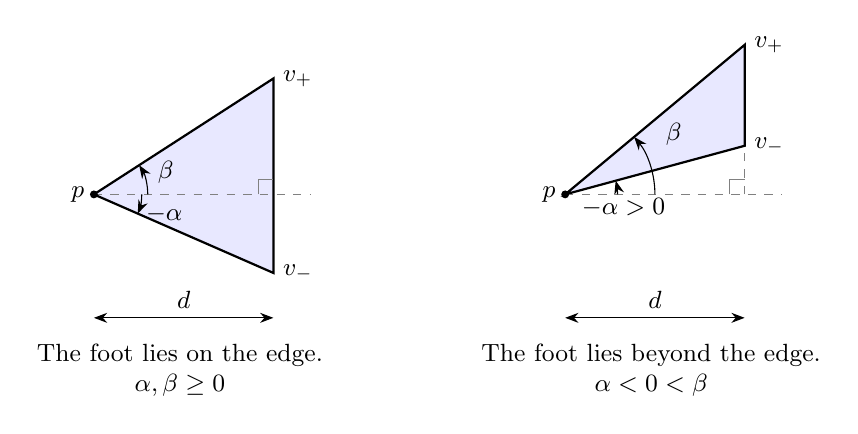
\begin{tikzpicture}[scale=.95,>=Stealth,font=\small]
\begin{scope}[shift={(0,0)}]
  \fill[blue!9] (0,0)--(2.4,-1.05)--(2.4,1.55)--cycle;
  \draw[thick] (0,0)--(2.4,-1.05)--(2.4,1.55)--cycle;
  \draw[dashed,gray] (0,0)--(2.9,0);
  \draw[gray] (2.2,0)--(2.2,.2)--(2.4,.2);
  \fill (0,0) circle (1.5pt) node[left] {$p$};
  \node[right] at (2.4,-1.05) {$v_-$};
  \node[right] at (2.4,1.55) {$v_+$};
  \draw[<->] (0,-1.65)--node[above] {$d$}(2.4,-1.65);
  \draw[->] (.72,0) arc[start angle=0,end angle=32.86,radius=.72];
  \node at (.96,.30) {$\beta$};
  \draw[->] (.64,0) arc[start angle=0,end angle=-23.63,radius=.64];
  \node at (.94,-.27) {$-\alpha$};
  \node[align=center] at (1.15,-2.35) {The foot lies on the edge.\\$\alpha,\beta\geq0$};
\end{scope}
\begin{scope}[shift={(6.3,0)}]
  \fill[blue!9] (0,0)--(2.4,.65)--(2.4,2)--cycle;
  \draw[thick] (0,0)--(2.4,.65)--(2.4,2)--cycle;
  \draw[dashed,gray] (0,0)--(2.9,0);
  \draw[dashed,gray] (2.4,0)--(2.4,.65);
  \draw[gray] (2.2,0)--(2.2,.2)--(2.4,.2);
  \fill (0,0) circle (1.5pt) node[left] {$p$};
  \node[right] at (2.4,.65) {$v_-$};
  \node[right] at (2.4,2) {$v_+$};
  \draw[<->] (0,-1.65)--node[above] {$d$}(2.4,-1.65);
  \draw[->] (1.20,0) arc[start angle=0,end angle=39.81,radius=1.20];
  \node at (1.45,.80) {$\beta$};
  \draw[->] (.70,0) arc[start angle=0,end angle=15.15,radius=.70];
  \node at (.78,-.18) {$-\alpha>0$};
  \node[align=center] at (1.15,-2.35) {The foot lies beyond the edge.\\$\alpha<0<\beta$};
\end{scope}
\end{tikzpicture}
\caption{Two possible Voronoi sectors, with the edge normal as angular
axis. In the right-hand sector both endpoints are above that axis,
so the lower endpoint parameter $\alpha$ is negative even though the
sector angle $\alpha+\beta$ is positive.}
\label{fig:signed-sectors}
\end{figure}


\subsection{Compatible flat-torus data and trace matching}

Let \(\Gamma\subset\R^2\) be a rank-two lattice and put
\(\mathbb T=\R^2/\Gamma\). Let \(N\geq1\) be an integer, let
\(v_1,\ldots,v_N\) be distinct points of \(\mathbb T\), and let
\(P\) be their full \(\Gamma\)-periodic lift. Suppose that the Voronoi
cells of \(P\) are bounded convex polygons with finitely many
face--edge incidences modulo \(\Gamma\). Assume that each incidence
has the sector form \eqref{geo:sector} and that, for one named constant
\(d_0>0\), every sector has \(d\geq d_0\). We call these
\emph{compatible periodic Voronoi data with lower edge distance \(d_0\)}.
This is conditional geometric data, not a separation assertion about
an arbitrary competitor.

The sectors partition the \(N\) cells modulo \(\Gamma\), up to their
boundary rays. Their total area is \(|\mathbb T|\), and their total
angle is \(2\pi N\): each convex cell has its site in its interior
because \(d_0>0\), so its sectors have total angle \(2\pi\).
These facts do not require an incidence bound.

Call a radius \(\eta>0\) admissible if it is smaller than the
injectivity radius of \(\mathbb T\) and, when \(N\geq2\), smaller
than half the minimum torus distance between distinct sites. Thus the
torus disks \(B(v_i,\eta)\) are embedded and pairwise disjoint; for
\(N=1\) there is no pairwise-distance condition. Write
\[
 \Omega_\eta=\mathbb T\setminus\bigcup_{i=1}^N B(v_i,\eta).
\]
In puncture limits we may further take \(\eta<d_0\), so every deleted
disk lies in its Voronoi cell. This restriction does not change a limit
as \(\eta\downarrow0\).

Fix compatible periodic Voronoi data with lower edge distance \(d_0\).
Let \(I\) be a finite or countable index set,
and choose integers \(k_i\geq6\), \(i\in I\); different indices
may have the same integer.  Suppose that
\[
 B\in C^1((0,\infty)),\qquad D_i\in C^1((0,\infty))
\]
satisfy the following assumptions:
\begin{equation}
 B(r)=-\log r+O(r^2),\qquad
 B'(r)=-1/r+O(r)
                    \quad(r\downarrow0),
 \label{dual:radial-origin}
\end{equation}
and, for every \(T_0>d_0\),
\begin{equation}
 \sum_{i\in I}\ \sup_{d_0\leq t\leq T_0}
 \bigl((1+k_i)|D_i(t)|+t|D_i'(t)|\bigr)<\infty.
 \label{dual:radial-sum}
\end{equation}
These are the exact inputs needed in the gluing and duality
argument.  The later radial construction will verify them
directly.

For a sector \eqref{geo:sector}, define \(t(\varphi)=d\sec\varphi\)
and
\begin{equation}
 H(r,\varphi)=B(r)+
       \sum_{i\in I}\left(\frac r{t(\varphi)}\right)^{k_i}
                                      D_i(t(\varphi)).
 \label{dual:trial}
\end{equation}
The same radial functions are used in every sector.

\begin{lemma}[Gluing and singular normalization]
\label{dual:gluing}
For compatible periodic Voronoi data on \(\mathbb T\) with \(N\geq1\)
distinct sites and lower edge distance \(d_0\), let \(I\) be finite or
countable, let \(k_i\geq6\) be integers with repetitions permitted,
and let \(B,D_i\in C^1((0,\infty))\) satisfy
\eqref{dual:radial-origin}--\eqref{dual:radial-sum}. The sector
functions \eqref{dual:trial} define a \(\Gamma\)-periodic
function \(H\) that is continuous off the sites and belongs to
\(H^1(\Omega_\eta)\) for every admissible \(\eta<d_0\). At every
site, uniformly in the angular variable,
\begin{equation}
 H=-\log r+O(r^2),\qquad
 \nabla H=-\frac{e_r}{r}+O(r).
 \label{dual:singularity}
\end{equation}
The gradient statement is sectorwise, and hence holds for the weak
gradient almost everywhere; no agreement of derivatives across sectors
is asserted.
In particular the constant term in \(H+\log r\) is zero.
\end{lemma}

\begin{proof}
Fix the finite collection of lifted polygons needed for one
torus. Their vertex radii are bounded by some \(T_0>d_0\). On each
closed sector, \(d_0\leq t\leq T_0\), \(r/t\leq1\), and
\(\tan\varphi\) is bounded.  The derivatives of a summand are
\[
 \partial_r\left[(r/t)^{k_i}D_i(t)\right]
       =\frac{k_i}{r}(r/t)^{k_i}D_i(t),
\]
and
\[
 \partial_\varphi\left[(r/t)^{k_i}D_i(t)\right]
       =\tan\varphi\,(r/t)^{k_i}
                         \bigl(tD_i'(t)-k_iD_i(t)\bigr).
\]
Assumption \eqref{dual:radial-sum} therefore gives uniform
convergence of the series and its first derivatives on each
closed sector away from its site.  Derivatives here are
sectorwise; derivatives across different sectors need not agree.

On a polygon edge, \(r=t\), so the trace is
\[
 B(r)+\sum_iD_i(r).
\]
The two adjacent sites have the same distance to that edge
point, and hence give the same trace.  On a ray from a site
to a vertex at distance \(r_v\), either neighboring sector has
\(t=r_v\) at its endpoint angle.  Both traces along the entire
ray are
\[
 B(r)+\sum_i(r/r_v)^{k_i}D_i(r_v).
\]
At a multiple vertex all incident sites have the same vertex
distance, so the edge traces also coincide there.  The recipe
is unchanged by period translations.

Thus all traces match.  Applying the Sobolev gluing property
to the finitely many sectors gives the asserted \(H^1\)
regularity off the holes.  No matching of normal derivatives
is required.

For \(r\leq d_0/2\), the fact that every \(k_i\geq6\), together
with \eqref{dual:radial-sum}, bounds the correction series by
\(O(r^6)\) and its gradient by \(O(r^5)\).  Combining these
bounds with \eqref{dual:radial-origin} proves
\eqref{dual:singularity}.
\end{proof}

The common notation \(D_i=b_i-u_i\), \(B=\sum_i u_i\) is one way
to supply these data.  In that notation the common edge trace
is simply \(\sum_i b_i(r)\).  The gluing argument itself only
uses \(B\) and \(D_i\).

\subsection{The exact dual identity}

Assume now that \(|\mathbb T|=N\). Let \(h\) be the mean-zero
distributional solution on \(\mathbb T\) of
\begin{equation}\label{dual:torus-potential}
 -\Delta h=2\pi\left(\sum_{i=1}^N\delta_{v_i}-1\right).
\end{equation}
The area condition is exactly the compatibility condition for this
equation. With the convention
\[
 \Gamma^*=\{k\in\R^2:k\cdot\gamma\in\Z
                     \text{ for every }\gamma\in\Gamma\},
\]
the Fourier mode \(e^{2\pi i k\cdot x}\) has eigenvalue
\(4\pi^2|k|^2\) under \(-\Delta\). The constant Fourier coefficient
of the right-hand side vanishes. Dividing its coefficient
at each nonzero \(k\in\Gamma^*\) by \(4\pi^2|k|^2\), and setting the
coefficient at zero to zero, gives a distributional solution. It is
unique because the kernel of the Laplacian on the torus consists of
constants. Define
\begin{equation}\label{dual:torus-energy}
 \mathcal W_{\mathbb T}(h)=\lim_{\eta\downarrow0}
 \left[
 \frac12\int_{\Omega_\eta}|\nabla h|^2\,\dd x+\pi N\log\eta
 \right],
\end{equation}
where the limit is taken through admissible radii. The local calculation
in Lemma~\ref{red:local}, applied in a torus chart, gives the finite
puncture limit. When \(\mathbb T=T_n\) and \(N=n\), this is exactly
\(\mathcal W_n(h)\) in \eqref{eq:torus-energy}.

For a sector \(S=S(d,\alpha,\beta)\), define
\begin{equation}
 \int_S^{\mathrm{ren}}|\nabla H|^2
 =\lim_{\eta\downarrow0}\left[
   \int_{S\cap\{r>\eta\}}|\nabla H|^2\,\dd x
                         +\theta(S)\log\eta\right].
 \label{dual:sector-ren}
\end{equation}
Lemma~\ref{dual:gluing} shows that this limit is finite.
Its counterterm uses the positive angle \(\theta(S)\), also
for a sector with a negative endpoint parameter.  Define
\begin{equation}
 J(S)=-2\pi\int_S H\,\dd x
             -\frac12\int_S^{\mathrm{ren}}|\nabla H|^2.
 \label{dual:sector-functional}
\end{equation}
The sectorwise estimates in the proof of Lemma~\ref{dual:gluing} also
show that these expressions are well defined on any individual sector
with \(d\geq d_0\) and the endpoint conditions in \eqref{geo:sector},
without first choosing a periodic tiling.

\begin{proposition}[Dual identity]
\label{dual:identity}
For compatible periodic Voronoi data on
\(\mathbb T=\R^2/\Gamma\) with \(N\geq1\) distinct sites, lower edge
distance \(d_0>0\), and \(|\mathbb T|=N\), let \(h\) be the mean-zero
potential \eqref{dual:torus-potential}. Let \(I\) be finite or countable,
let \(k_i\geq6\) be integers with repetitions permitted, and let
\(B,D_i\in C^1((0,\infty))\) satisfy
\eqref{dual:radial-origin}--\eqref{dual:radial-sum}. Let \(H\) be the
function supplied by Lemma~\ref{dual:gluing}. Then
\begin{equation}
 \mathcal W_{\mathbb T}(h)
   =\sum_S J(S)+
              \frac12\int_{\mathbb T}|\nabla(h-H)|^2\,\dd x
   \geq\sum_S J(S).
 \label{dual:energy-bound}
\end{equation}
The sum runs over all face--edge incidences in one torus.
No incidence bound or square-torus separation hypothesis is imposed.
\end{proposition}

\begin{proof}
Apply Lemma~\ref{red:local} in a local chart to \(-\nabla h\).
Near each site, \(h=-\log r+a_i+O(r)\) and
\(\nabla h=-e_r/r+O(1)\). Thus both \(h\) and \(H\) have singular
gradient \(-e_r/r\).
Their difference has square-integrable gradient.  Also
\eqref{dual:singularity} implies that
\[
 I_{\mathrm{ren}}(H)=
 \lim_{\eta\downarrow0}\left[
       \int_{\Omega_\eta}|\nabla H|^2+2\pi N\log\eta\right]
\]
exists. For admissible \(\eta<d_0\), the punctured sectors partition
\(\Omega_\eta\) up to their boundaries. The sector angles sum to
\(2\pi N\), so \(I_{\mathrm{ren}}(H)\) equals the sum of
\eqref{dual:sector-ren}.

Green's identity, with \(h\) smooth on the punctured torus and
\(H\in H^1(\Omega_\eta)\), gives
\[
 \int_{\Omega_\eta}\nabla h\cdot\nabla H
  =-2\pi\int_{\Omega_\eta}H
     +\sum_i\int_{\partial B(v_i,\eta)}
                          H\,\partial_{\boldsymbol n}h.
\]
The outward hole normal gives
\(\partial_{\boldsymbol n}h=1/\eta+O(1)\).
The zero constant term in \eqref{dual:singularity} therefore
gives
\[
 \int_{\Omega_\eta}\nabla h\cdot\nabla H
      =-2\pi\int_{\mathbb T}H-2\pi N\log\eta+o(1).
\]
Expanding \(|\nabla(h-H)|^2\), inserting this identity, and
taking the puncture limit proves
\[
 \mathcal W_{\mathbb T}(h)
   =-2\pi\int_{\mathbb T}H-\frac12I_{\mathrm{ren}}(H)
          +\frac12\int_{\mathbb T}|\nabla(h-H)|^2.
\]
Partitioning the first two terms into sectors proves
\eqref{dual:energy-bound}.
\end{proof}

If the gradient hypotheses were unchanged but the value expansion were
instead \(H=-\log r+c_i+o(1)\) at \(v_i\), the right-hand side of the
last identity would contain the additional term
\(2\pi\sum_i c_i\).  This explains why the zero constant term
in the radial construction is part of the normalization.

For a square-torus minimizer, Lemma~\ref{geo:voronoi} supplies the
compatible data with \(\Gamma=\sqrt n\,\Z^2\), \(N=n\), and
\(d_0=d_*=r_*/2=1/(2\sqrt\pi)\). Its torus has area \(n\), so
Proposition~\ref{dual:identity} applies with
\(\mathcal W_{\mathbb T}=\mathcal W_n\). The triangular application
in the next section supplies its own period and sectors and does not
use a square-torus minimizer.

\subsection{From scalar estimates to configuration bounds}

The two scalar bounds below control ordinary and signed sectors by
different arguments. Once they yield an affine lower bound for each
sector, the dual identity and the incidence count give the energy
bound. We formulate this implication for compatible flat tori first;
separation of a square-torus minimizer then removes the geometric
hypotheses from the finite-volume comparison.

\begin{lemma}[Signed endpoint parameters]
\label{dual:signed-endpoints}
Let \(K<0\) and \(d_0>0\). For each \(d\geq d_0\), let
\(G(d,\cdot)\) be an even locally integrable real function on \(\R\),
and put
\[
 g_d(x)=\int_0^xG(d,s)\,\dd s.
\]
Suppose that, for every \(d\geq d_0\),
\begin{equation}
 2g_d(x)\geq K\quad(x\geq0),\qquad
 \int_0^\infty\max\{0,-G(d,s)\}\,\dd s\leq-K.
 \label{dual:scalar-input}
\end{equation}
Then, for every \(d\geq d_0\) and every pair \(\alpha,\beta\) with
\(|\alpha|,|\beta|<\pi/2\) and \(\alpha+\beta>0\),
\begin{equation}
 g_d(d\tan\alpha)+g_d(d\tan\beta)\geq K.
 \label{dual:signed-bound}
\end{equation}
\end{lemma}

\begin{proof}
Evenness of \(G(d,\cdot)\) makes \(g_d\) odd. If
\(\alpha,\beta\geq0\), the first inequality in
\eqref{dual:scalar-input} bounds each term in
\eqref{dual:signed-bound} below by \(K/2\).

If \(\alpha<0\), set
\[
 u=-d\tan\alpha,\qquad v=d\tan\beta.
\]
The inequality \(\alpha+\beta>0\) gives \(\beta>-\alpha>0\).
Since the tangent is increasing on \((-\pi/2,\pi/2)\), we have
\(0<u<v\). Oddness and the second inequality in
\eqref{dual:scalar-input} give
\[
 \begin{aligned}
 g_d(d\tan\alpha)+g_d(d\tan\beta)
 &=g_d(v)-g_d(u)=\int_u^vG(d,s)\,\dd s\\
 &\geq-\int_0^\infty\max\{0,-G(d,s)\}\,\dd s\geq K.
 \end{aligned}
\]
The case \(\beta<0\) is symmetric. Both endpoints cannot be negative
because their sum is positive, so these cases are exhaustive.
\end{proof}

\begin{proposition}[From sector bounds to energy bounds]
\label{dual:assembly}
Let \(d_0>0\), let \(I\) be finite or countable, let \(k_i\geq6\)
be integers with repetitions permitted, and let
\(B,D_i\in C^1((0,\infty))\) satisfy
\eqref{dual:radial-origin} and \eqref{dual:radial-sum} with
this lower distance \(d_0\). For every sector \eqref{geo:sector} with
\(d\geq d_0\), use these same radial data in \eqref{dual:trial} and
let \(J(S)\) be the functional \eqref{dual:sector-functional}.
Suppose that \(K\leq0\) and \(\lambda,\mu\in\R\) satisfy
\begin{equation}
 \begin{aligned}
 J(S(d,\alpha,\beta))
 &\geq K+\lambda A(S(d,\alpha,\beta))\\
 &\qquad+\mu\theta(S(d,\alpha,\beta)),
 \end{aligned}
 \label{dual:sector-input}
\end{equation}
for every \(d\geq d_0\), \(|\alpha|,|\beta|<\pi/2\), and
\(\alpha+\beta>0\).

\emph{Compatible tori.}
Let \(\mathbb T=\R^2/\Gamma\) have area \(N\), where \(N\geq1\)
is an integer. Suppose \(N\) distinct sites supply compatible periodic
Voronoi data with lower edge distance \(d_0\) and at most \(6N\)
face--edge sectors. Their mean-zero potential
\eqref{dual:torus-potential} satisfies
\begin{equation}\label{dual:compatible-bound}
 \mathcal W_{\mathbb T}(h)\geq N(6K+\lambda+2\pi\mu).
\end{equation}

\emph{All square-torus configurations.}
Assume in addition \(d_0\leq d_*=1/(2\sqrt\pi)\). For every
integer \(n\geq2\) and every configuration of \(n\) distinct
points \(v_1,\ldots,v_n\) on \(T_n=\R^2/(\sqrt n\,\Z^2)\), let \(h\)
be the mean-zero solution of
\[
 -\Delta h=2\pi\left(\sum_{i=1}^n\delta_{v_i}-1\right).
\]
Then its puncture-first energy \eqref{eq:torus-energy}, with embedded
and pairwise disjoint punctures, satisfies
\begin{equation}
 \mathcal W_n(h)\geq n(6K+\lambda+2\pi\mu).
 \label{dual:all-configurations}
\end{equation}
More generally, if a periodic locally integrable field \(E\) on \(T_n\)
satisfies, distributionally,
\[
 \operatorname{div}E=2\pi\left(\sum_{i=1}^n\delta_{v_i}-1\right),
 \qquad \operatorname{curl}E=0,
\]
then \(E=-\nabla h+c\) for a constant \(c\in\R^2\), and its energy
with the same punctures and counterterm obeys
\[
 \mathcal E_{T_n}(E)=\mathcal W_n(h)+\frac n2|c|^2
                    \geq n(6K+\lambda+2\pi\mu).
\]
The energy identity remains valid after applying the same fixed
orthogonal rotation to both fields.
\end{proposition}

\begin{proof}
For compatible data, the sectors have total area \(N\) and total
angle \(2\pi N\). Write \(M_0\leq6N\) for their number.
Proposition~\ref{dual:identity} and \eqref{dual:sector-input} give
\[
 \begin{aligned}
 \mathcal W_{\mathbb T}(h)
 &\geq\sum_S J(S)\\
 &\geq M_0K+\lambda N+2\pi\mu N\\
 &\geq N(6K+\lambda+2\pi\mu).
 \end{aligned}
\]
The last inequality uses \(M_0\leq6N\) and \(K\leq0\); it includes
\(K=0\), when both terms involving \(K\) vanish.

Now assume \(d_0\leq d_*\) and fix \(n\geq2\).
Lemma~\ref{geo:existence} supplies a minimizing configuration of
distinct points, with potential \(h_{\min}\).
Lemma~\ref{geo:separation} separates its full periodic lift by
\(r_*=1/\sqrt\pi\). Lemma~\ref{geo:voronoi} then gives at most
\(6n\) sectors, each with edge distance at least \(d_*\geq d_0\).
These are compatible data on \(T_n\), so
\eqref{dual:compatible-bound} applies to \(h_{\min}\).
Every other distinct configuration has energy at least
\(\mathcal W_n(h_{\min})\), proving
\eqref{dual:all-configurations} without a separation assumption on
that configuration.

Equation~\eqref{red:harmonic} applies to the displayed divergence and
curl conditions and gives the constant harmonic component and its
exact energy penalty. A fixed orthogonal rotation preserves the
squared norm and the puncture counterterm, giving the last assertion.
\end{proof}

The next section chooses particular radial data and exact constants
\(K<0,\lambda,\mu\). For these data, the primitive identity
\eqref{cal:sector-primitive} and the two scalar bounds yield
\[
 J(S)\geq K+\lambda A(S)+\mu\theta(S)
\]
for every relevant sector. Proposition~\ref{cal:scalar-to-torus}
applies the compatible-torus conclusion to this construction and
identifies \(6K+\lambda+2\pi\mu\) with the triangular energy.
Section~\ref{sec:conclusion} uses the square-torus conclusion, whose
minimizer argument has already removed the separation hypothesis.

\section{Calibration on the triangular cell}\label{cal:section}\label{sec:calibration}

We construct the radial functions used by the Voronoi test potential.
The potential has the same gradient as the triangular Green function
on a regular hexagon, while its energy on every other sector reduces
to two scalar estimates.  The continuation outside that hexagon is
auxiliary; its explicit form makes those estimates accessible to
interval arithmetic.

\subsection{The local triangular Green function}
Set
\begin{equation}\label{cal:geometry}
 a=\sqrt{\frac{2}{\sqrt3}},\qquad p=\frac a2,\qquad
 R_0=\frac{2p}{\sqrt3},\qquad x_0=\frac{R_0}{2}.
\end{equation}
Thus $p$ and $R_0$ are the inradius and circumradius of the covolume-one
triangular Voronoi hexagon, and $x_0=p\tan(\pi/6)$.
Identify the plane with $\mathbb C$, and write
$\partial_z=(\partial_x-i\partial_y)/2$, with a nearest lattice point on the
positive real axis.  For $m\ge1$ put
\begin{equation}\label{cal:coefficients}
 k_m=6m,\qquad
 c_m=\frac1{k_m}\sum_{z\in\Lambda_\triangle\setminus\{0\}}z^{-k_m}.
\end{equation}
These sums converge absolutely and are real by reflection symmetry.
We also introduce an auxiliary index $0$, with $k_0=6$.
It is distinct from index $1$: both exponents equal $6$, but they will
carry different radial functions.

\begin{lemma}\label{cal:green-expansion}
The mean-zero triangular Green function has the expansion
\begin{equation}\label{cal:green-series}
 h_\triangle(z)=-\log|z|+C_\triangle+\frac{\pi|z|^2}{2}
                 +\sum_{m\ge1}c_m\operatorname{Re}(z^{6m}),
 \qquad 0<|z|<a,
\end{equation}
where $C_\triangle$ is its regular part at the origin.  The series and
all of its derivatives converge locally away from $|z|=a$.
\end{lemma}
\begin{proof}
Away from the lattice, $\Delta h_\triangle=2\pi$, so
$2\partial_z^2h_\triangle$ is a meromorphic elliptic function.  Its double
pole at each lattice point has principal part $(z-\lambda)^{-2}$.
Subtract the absolutely locally convergent Weierstrass series
\[
 \wp(z)=\frac1{z^2}+\sum_{\lambda\ne0}
       \bigl((z-\lambda)^{-2}-\lambda^{-2}\bigr).
\]
The difference is holomorphic and periodic, hence constant.  If
$\omega=e^{\pi i/3}$, invariance of $h_\triangle$ under $z\mapsto\omega z$
implies that its second complex derivative transforms by $\omega^{-2}$;
the same is true of $\wp$.  Their constant difference must therefore vanish.
Expanding each summand for $|z|<a$ gives
\[
 \wp(z)=z^{-2}+\sum_{j\ge1}(j+1)z^j
                         \sum_{\lambda\ne0}\lambda^{-j-2}.
\]
Rotation makes the inner sum zero unless $j+2$ is a multiple of $6$.
Twice complex differentiation of the right side of
\eqref{cal:green-series} gives this series, because
$k_m(k_m-1)c_m=(k_m-1)\sum\lambda^{-k_m}$.
The difference is a real harmonic affine function after subtracting
$\pi|z|^2/2$; rotation removes its linear part and leaves $C_\triangle$.
Normal convergence follows either from this power series or from the
absolutely convergent lattice sums on every smaller disk.
\end{proof}

\subsection{Matching the regular hexagon}
Write $\gamma(r)=-\log r+\pi r^2/2$ for $r>0$.
We first choose the radial data on the regular hexagon, where the test
potential must equal $h_\triangle-C_\triangle$.  In a sector whose
outward normal is the positive real axis, the edge has distance $p$
and the endpoint angles are $\pm\pi/6$.  At an edge point of radius
$t=p\sec\varphi$,
\[
 p+i\sqrt{t^2-p^2}=te^{i|\varphi|}.
\]
The boundary value of the $m$th Green-function mode is therefore
$c_mt^{k_m}\cos(k_m\varphi)$.  Expressing it as a function of the
radius gives the polynomial
\begin{equation}\label{cal:edge-polynomial}
 V_m(r)=c_m\sum_{j=0}^{k_m/2}(-1)^j\binom{k_m}{2j}
                          p^{k_m-2j}(r^2-p^2)^j,
 \qquad p\le r\le R_0.
\end{equation}
On either vertex ray, the same mode equals
$(-1)^mc_mr^{k_m}$, since $k_m\pi/6=m\pi$.  This is the radial
baseline we use for that mode inside the hexagon.  The correction in
\eqref{dual:trial} then recovers the angular dependence exactly:
\[
 (-1)^mc_mr^{k_m}
   +(r/t)^{k_m}\bigl(V_m(t)-(-1)^mc_mt^{k_m}\bigr)
       =c_mr^{k_m}\cos(k_m\varphi).
\]
Thus the edge data $b_m=V_m$ and the vertex-ray baseline determine the
desired potential on each regular sector.  Its remaining part $\gamma$
is already radial and needs no correction there.

\subsection{Continuation to arbitrary sectors}
Other Voronoi sectors can have edge radii below $p$ or above $R_0$.
We now extend the radial data to those radii, keeping two derivatives
and making the correction vanish beyond a fixed radius.  The assembled
potential is required to agree with $h_\triangle-C_\triangle$ only
inside the regular hexagon; the continuation is chosen for the scalar
estimates, not as an extension of that Green function.

Define the clipped polynomial
\[
 S(y)=\begin{cases}
 0,&y\le0,\\
 10y^3-15y^4+6y^5,&0<y<1,\\
 1,&y\ge1.
 \end{cases}
\]
Let $h_s=3/40$ and $c=3/50$.  For $0\le z\le h_s$ put
\[
 P(z)=z-\frac{6z^3}{h_s^2}+\frac{8z^4}{h_s^3}-\frac{3z^5}{h_s^4},\qquad
 Q(z)=\frac{z^2}{2}-\frac{3z^3}{2h_s}
                       +\frac{3z^4}{2h_s^2}-\frac{z^5}{2h_s^3}.
\]
For a function $V$ with two left derivatives at $R_0$, its continuation
is defined for $r\ge R_0$ by
\begin{equation}\label{cal:continuation}
 (\mathcal HV)(r)=
 \begin{cases}
 V(R_0)+P(r-R_0)V'(R_0)+Q(r-R_0)V''(R_0),&r\le R_0+h_s,\\
 V(R_0),&r>R_0+h_s.
 \end{cases}
\end{equation}
Indeed $(P,P',P'')(0)=(0,1,0)$ and
$(Q,Q',Q'')(0)=(0,0,1)$; all six values at $h_s$ vanish.
Thus this operation preserves two derivatives at $R_0$ and joins a
constant with two derivatives at $R_0+h_s$.

Define $b_0=\gamma$ up to $R_0$, continued by
\eqref{cal:continuation}.  For $m\ge1$, set $b_m=V_m$ on $[p,R_0]$
and use $\mathcal HV_m$ above $R_0$.
Below $p$ put
\begin{equation}\label{cal:inner-continuation}
 b_m(r)=\begin{cases}
 0,&0<r\le p-c,\\
 S((r-p+c)/c)\bigl(T_{0m}+T_{1m}(r-p)+T_{2m}(r-p)^2\bigr),&p-c<r<p,
 \end{cases}
\end{equation}
where
\[
 \begin{split}
 T_{0m}&=c_mp^{k_m},\\
 T_{1m}&=-\frac{k_m(k_m-1)}pT_{0m},\\
 T_{2m}&=\frac{k_m(k_m-1)}{p^2}
             \left(\frac{(k_m-2)(k_m-3)}6-\frac12\right)T_{0m}.
 \end{split}
\]
Direct differentiation of \eqref{cal:edge-polynomial} gives
$T_{0m}=V_m(p)$, $T_{1m}=V_m'(p)$, and $2T_{2m}=V_m''(p)$.
Consequently every $b_i$ is $C^2$ away from the origin.

Now define
\[
 U_m(r)=(-1)^mc_mr^{k_m}\bigl(1-S((r-R_0)/(1/10))\bigr),\qquad
 \tau(r)=S\left(\frac{r-R_0-1/1000}{3/40}\right),
\]
and set
\begin{equation}\label{cal:radial-data}
 \begin{split}
 u_0&=(1-\tau)\gamma+\tau b_0,\qquad
 u_m=(1-\tau)U_m+\tau b_m\quad(m\ge1),\\
 B&=\sum_{i\ge0}u_i,\qquad D_i=b_i-u_i,\qquad
 l=R_0+\frac{19}{250}.
 \end{split}
\end{equation}
Here the auxiliary mode $0$ lets the radial part $\gamma$ join its
constant continuation by the same correction mechanism as the other
modes.  Its exponent $k_0=6$ makes this correction vanish at the pole
without changing the singular normalization.  The coefficient
estimates proved below justify the sums and their
first three derivatives on every open spline interval.  In particular,
$B,D_i$ are $C^2$ and piecewise $C^3$ away from zero.  Near zero,
$B=\gamma+\sum_{m\ge1}(-1)^mc_mr^{k_m}$; normal convergence of
\eqref{cal:green-series} therefore gives
\begin{equation}\label{cal:radial-endpoints}
 \begin{gathered}
 B(r)=-\log r+O(r^2),\qquad B'(r)=-1/r+O(r)\quad(r\downarrow0),\\
 D_i(r)=0,\qquad B(r)=B(l)\quad(r\ge l).
 \end{gathered}
\end{equation}
The fixed radial data also satisfy \eqref{dual:radial-sum} for every
$d_0>0$.  Indeed, there are only finitely many retained modes, while
for the omitted modes \eqref{tail:mode-derivative-bound} and the
vanishing of $D_i$ beyond $l$ bound the summand on $[d_0,T_0]$ by
$(1+k_i+T_0)w_{k_i}$.  The explicit geometric terms in
\eqref{tail:w-definition} make this series summable.  This conclusion
uses the analytic mode bounds, not the later finite-core estimates.

For a sector with edge distance $d$ and endpoint angles $-\alpha<\beta$,
write $t(\varphi)=d\sec\varphi$ and use the test potential
\begin{equation}\label{cal:trial-potential}
 H(r,\varphi)=B(r)+\sum_{i\ge0}
                   \left(\frac r{t(\varphi)}\right)^{k_i}D_i(t(\varphi)),
 \qquad 0<r<t(\varphi),\quad -\alpha<\varphi<\beta.
\end{equation}
At the edge its trace is $\sum_i b_i(t)$; at a ray ending at a vertex of
radius $r_v$ its trace is $B(r)+\sum_i(r/r_v)^{k_i}D_i(r_v)$.
These expressions explain both trace matching conditions in the glued
Voronoi construction.

\subsection{The sector integral}
The following formulas separate radial integration from sector geometry.
For $t>0$ define
\begin{equation}\label{cal:radial-integrals}
 \begin{split}
 B_1(t)&=B'(t)+1/t,\qquad S_1(t)=\int_0^t B(r)r\,dr,\\
 S_2(t)&=\int_0^t\bigl(-2B_1(r)+rB_1(r)^2\bigr)\,dr,\\
 H_k(t)&=t^{-k}\int_0^tB_1(r)r^k\,dr,\qquad
 Q_i(t)=tD_i'(t)-k_iD_i(t).
 \end{split}
\end{equation}
Here $H_k$ is indexed by the exponent, so the two modes with exponent
six use the same $H_6$.  They remain separate in every sum involving $D_i$.
Put
\begin{equation}\label{cal:f0-e}
 \begin{split}
 f_0(t)={}&-2\pi\left(S_1(t)+t^2\sum_i\frac{D_i(t)}{k_i+2}\right)\\
 &-\frac12\Biggl(\log t+S_2(t)
   +\sum_i\bigl(-2D_i(t)+2k_iD_i(t)H_{k_i}(t)\bigr)\\
 &\qquad+\sum_{i,j}\frac{k_ik_j}{k_i+k_j}D_i(t)D_j(t)\Biggr),\\
 e(t)={}&\frac12\sum_{i,j}\frac{Q_i(t)Q_j(t)}{k_i+k_j}.
 \end{split}
\end{equation}
All sums here and below include index $0$.
The angular coefficient is nonnegative, since
\begin{equation}\label{cal:positive-kernel}
 e(t)=\frac12\int_0^1
          \left(\sum_iQ_i(t)v^{k_i}\right)^2\frac{dv}{v}\ge0.
\end{equation}

Let $J$ denote the sector contribution to the dual energy,
\[
 J=-2\pi\int_{\rm sector}H
            -\frac12\int_{\rm sector}^{\rm ren}|\nabla H|^2,
\]
where the renormalized integral adds $(\alpha+\beta)\log\eta$ before
letting the radial exclusion $\eta$ tend to zero.  Then
\begin{equation}\label{cal:angle-density}
 J=\int_{-\alpha}^{\beta}
          \bigl(f_0(d\sec\varphi)-\tan^2\varphi\,e(d\sec\varphi)\bigr)
                                                                  \,d\varphi.
\end{equation}
To verify this identity, differentiate \eqref{cal:trial-potential}:
\[
 H_r=-\frac1r+B_1(r)+\sum_i\frac{k_i}{r}(r/t)^{k_i}D_i(t),\qquad
 H_\varphi=\tan\varphi\sum_i(r/t)^{k_i}Q_i(t).
\]
The source integral gives $S_1+t^2\sum_iD_i/(k_i+2)$.
The radial square contributes $\log t+S_2$, its cross terms contribute
$-2D_i+2k_iD_iH_{k_i}$, and its quadratic terms have coefficient
$k_ik_j/(k_i+k_j)$.  Integrating the angular square gives
$\tan^2\varphi\sum Q_iQ_j/(k_i+k_j)$.  These are precisely
\eqref{cal:f0-e}.  The estimates below permit termwise integration.

\subsection{Subtracting area and angle}
Given real constants $\lambda,\mu$, define
\begin{equation}\label{cal:primitive}
 \begin{split}
 f(t)&=f_0(t)-\lambda t^2/2-\mu,\qquad t=\sqrt{d^2+s^2},\\
 G(d,s)&=\frac d{t^2}f(t)-\frac{s^2}{dt^2}e(t),\qquad
 g_d(x)=\int_0^xG(d,s)\,ds\quad(d>0,\ x\in\mathbb R).
 \end{split}
\end{equation}
The evenness of $G$ in $s$ makes $g_d$ odd.  If $A$ is the sector area
and $\theta=\alpha+\beta$, substitution $s=d\tan\varphi$ in
\eqref{cal:angle-density} gives
\begin{equation}\label{cal:sector-primitive}
 J-\lambda A-\mu\theta
       =g_d(d\tan\alpha)+g_d(d\tan\beta).
\end{equation}
This identity holds for signed endpoint angles; only
$|\alpha|,|\beta|<\pi/2$ and $\alpha+\beta>0$ are required.

We choose $\lambda,\mu$ so that the adjusted primitive is stationary
at the regular sector $(d,x)=(p,x_0)$, and set $K$ to twice its value
there.  The exact choices are
\begin{equation}\label{cal:constants}
 \begin{split}
 \lambda=\frac1{px_0}\biggl[&\frac p{x_0}\bigl(f_0(R_0)-f_0(p)\bigr)
                 -\frac{x_0}{p}e(R_0)\\
 &+p\int_0^{x_0}\frac{f_0(\sqrt{p^2+s^2})-f_0(p)}{s^2}\,ds
                 +\frac1p\int_0^{x_0}e(\sqrt{p^2+s^2})\,ds\biggr],\\
 \mu={}&f_0(R_0)-\frac13e(R_0)-\lambda R_0^2/2,\qquad
 K=2g_p(x_0).
 \end{split}
\end{equation}
The first integrand extends continuously to $s=0$ with value
$f_0'(p)/(2p)$.

\begin{lemma}\label{cal:stationarity}
For the constants \eqref{cal:constants},
$\nabla_{d,x}g_d(x)=0$ at $(p,x_0)$.
\end{lemma}
\begin{proof}
Let $g_d^0$ denote the primitive before subtracting area and angle.
For fixed $u=\pi/6$, differentiation in the angle representation gives
\[
 \left.\frac d{dd}g_d^0(d\tan u)\right|_{d=p}
 =\int_0^{x_0}\frac{f_0'(t)-s^2e'(t)/p^2}{t}\,ds,
 \qquad t=\sqrt{p^2+s^2}.
\]
Set $V(s)=f_0(t)-f_0(p)$.  Since $V(s)=O(s^2)$, integration by parts
has no boundary term at zero and yields
\[
 \int_0^{x_0}\frac{f_0'(t)}t\,ds
       =\frac{f_0(R_0)-f_0(p)}{x_0}
                         +\int_0^{x_0}\frac{V(s)}{s^2}\,ds,
\]
whereas
\[
 \int_0^{x_0}\frac{s^2e'(t)}{p^2t}\,ds
       =\frac{x_0e(R_0)}{p^2}-\frac1{p^2}\int_0^{x_0}e(t)\,ds.
\]
The difference is the bracket in \eqref{cal:constants} divided by $p$,
hence equals $\lambda x_0$.
The subtracted area along $x=d\tan u$ is $\lambda d^2\tan u/2$;
its derivative at $p$ is also $\lambda x_0$, and the subtracted angle is
constant.  Thus the derivative of $g_d(d\tan u)$ vanishes there.
Finally $\partial_xg_p(x_0)=G(p,x_0)=0$ by the definition of $\mu$,
because $x_0^2/p^2=1/3$.  The fixed-angle derivative is
$\partial_d+(x_0/p)\partial_x$, so $\partial_d$ vanishes as well.
\end{proof}

\begin{lemma}\label{cal:energy-identity}
The calibrated constants satisfy
\begin{equation}\label{cal:triangular-energy}
 W(E_\triangle)=6K+\lambda+2\pi\mu.
\end{equation}
\end{lemma}
\begin{proof}
Take $\mathbb T=\R^2/\Lambda_\triangle$ and $N=1$.  Its regular
Voronoi hexagon supplies six compatible sectors with $d=p$ and
$\alpha=\beta=\pi/6$.  The radial normalization and summability
proved above supply the hypotheses of Proposition~\ref{dual:identity}
with $d_0=p$, and the torus has area one.  This application uses no
square-torus minimizer or incidence theorem.

On each sector $p\le t\le R_0$,
$u_0(r)=\gamma(r)$ and $u_m(r)=(-1)^mc_mr^{k_m}$ for $r\le t$.
The edge trace and mode cancellation established above therefore give
\[
 H(r,\varphi)=\gamma(r)+\sum_{m\ge1}c_mr^{k_m}\cos(k_m\varphi)
             =h_\triangle-C_\triangle.
\]
All six normals differ by multiples of $\pi/3$, which leaves these
cosines unchanged.  Hence $\nabla H=\nabla h_\triangle$ and the
nonnegative square in \eqref{dual:energy-bound} is zero.
Each sector has area $1/6$ and angle $\pi/3$; its right side in
\eqref{cal:sector-primitive} is $2g_p(x_0)=K$.
Summing the six contributions gives the cell energy
$6K+\lambda+2\pi\mu$.  Lemma~\ref{red:periodic-average} identifies
this cell energy with $W(E_\triangle)$, proving
\eqref{cal:triangular-energy}.
\end{proof}

\subsection{The two scalar estimates needed by the geometry}
The remaining analytic task is to establish
\begin{equation}\label{cal:scalar-bounds}
 \begin{gathered}
 K<0,\qquad 2g_d(x)\ge K\quad(d\ge b,\ x\ge0),\qquad b=\frac{28209}{100000},\\
 \int_0^\infty\max\{0,-G(d,s)\}\,ds\le-K\quad(d\ge b).
 \end{gathered}
\end{equation}
The rational endpoint $b=28209/100000$ is below the geometric
threshold $d_*=1/(2\sqrt\pi)$. Thus the domain $d\ge b$ covers all
edge distances supplied by the separated-minimizer geometry; the
elementary comparison is justified in Section~\ref{sec:conclusion}.

The second estimate is essential when the perpendicular from a point
to a Voronoi edge falls outside that edge.  Its role is made precise
in the following implication, which completes the geometric part of
the argument once \eqref{cal:scalar-bounds} has been certified.

\begin{proposition}\label{cal:scalar-to-torus}
Assume \eqref{cal:scalar-bounds} for the functions and constants just
constructed.  Let $\mathbb T=\R^2/\Gamma$ be a flat torus of area $N$,
where $N\ge1$ is an integer, and let $v_1,\ldots,v_N$ be distinct
sites.  Suppose their full periodic lift gives compatible periodic
Voronoi data with lower edge distance $d_0=b$ and at most $6N$
face-edge sectors.  Let $h$ be the mean-zero potential
\eqref{dual:torus-potential}, with energy
$\mathcal W_{\mathbb T}(h)$ defined by \eqref{dual:torus-energy}.
Then
\[
 \mathcal W_{\mathbb T}(h)\ge NW(E_\triangle).
\]
\end{proposition}
\begin{proof}
The radial normalization and compact summability established above
supply the radial hypotheses of Proposition~\ref{dual:assembly}
with $d_0=b$.  Evenness of $G$ and \eqref{cal:scalar-bounds} supply
the hypotheses of Lemma~\ref{dual:signed-endpoints} at this same
lower distance.  Combining its conclusion with
\eqref{cal:sector-primitive} gives
\[
 J(S)\ge K+\lambda A(S)+\mu\theta(S)
\]
for every sector with $d\ge b$, including the signed endpoint cases.
The compatible-torus conclusion \eqref{dual:compatible-bound} now gives
\[
 \mathcal W_{\mathbb T}(h)\ge N(6K+\lambda+2\pi\mu)
                         =NW(E_\triangle).
\]
The equality is the exact triangular calibration
\eqref{cal:triangular-energy}, not a numerical estimate of the
triangular energy.
\end{proof}

\section{Infinite-mode truncation and error propagation}
\label{tail:section}\label{sec:tails}

This section supplies analytic estimates for the modes omitted after
$m=38$.  We use the radial functions $b_m,U_m,u_m,B,D_m$ of the preceding
construction, with
\[
 \begin{gathered}
 a=\sqrt{2/\sqrt3},\qquad p=a/2,\qquad R_0=a/\sqrt3,\\
 b=\frac{28209}{100000},\qquad h_s=\frac{3}{40},\qquad
 c=\frac{3}{50},\qquad l=R_0+\frac{19}{250}.
 \end{gathered}
\]
Thus $k_0=6$, $k_m=6m$ for $m\geq1$, and
\[
 c_m=\frac1{k_m}\sum_{z\in\Lambda_\triangle\setminus\{0\}}z^{-k_m}.
\]
Tildes will always mean that the modes $m\geq39$ have been omitted;
the index-zero term is retained.  Differences between a full quantity
and its truncation are denoted by $\Delta$.
Our goal is an absolute error below $10^{-11}$ for $f_0,e$ and their
first two derivatives on $[b,l]$, conditional on the retained-mode
bounds verified in Section~\ref{sec:computation}.

\subsection{Coefficient estimates}
\label{tail:coefficients}

Write a lattice point as
$z=a(n+q/2+i\sqrt3 q/2)$, with $(n,q)\in\Z^2$.  Then
\[
 |z/a|^2=n^2+nq+q^2\geq\frac34\max(|n|,|q|)^2.
\]
There are $8v$ integer pairs with $\max(|n|,|q|)=v$.  For every
$d=6m\geq6$ and every positive integer $D$, the sum outside the square
$|n|,|q|\leq D$, before multiplication by $a^{-d}$, is therefore at most
\begin{equation}
 8(4/3)^{d/2}\sum_{v>D}v^{1-d}
 \leq 8(4/3)^{d/2}\frac{D^{2-d}}{d-2}.
 \label{tail:coefficient-square}
\end{equation}
The last inequality follows by comparison with the integral from $D$
to infinity.  The first shell has six points with squared norm $1$
and two with squared norm $3$.  Moreover,
\[
 \sum_{v\geq2}v^{1-d}
 \leq 2^{1-d}+\int_2^\infty x^{1-d}\,\dd x
 =2^{1-d}\left(1+\frac2{d-2}\right)
 \leq3\,2^{1-d}.
\]
It follows that, for $d=k_m\geq12$,
\begin{equation}
 |c_m|\leq\frac{1}{d a^d}
 \left(6+2\,3^{-d/2}+24(4/3)^{d/2}2^{1-d}\right)
 \leq\frac7{d a^d}.
 \label{tail:coefficient-uniform}
\end{equation}
Indeed, the bracket equals $6+50/729<7$ at $d=12$, and its two
nonconstant terms decrease with $d$.  The finite coefficient
enclosures may use \eqref{tail:coefficient-square} with $D=256$ for
$m=1$ and $D=48$ for $2\leq m\leq38$, including the factor
$1/(k_m a^{k_m})$.  Reflection symmetry makes each coefficient real.

\subsection{Uniform derivative bounds for omitted modes}
\label{tail:radial-derivatives}

For $k=6m\geq234$, define the rational number
\begin{equation}
 w_k=10^6\left(
 30k^2(13/20)^k+3\cdot10^6 k^3 2^{-k}
 +5600k^5(3/5)^k+7\cdot10^{11}k^2(289/500)^k
 \right).
 \label{tail:w-definition}
\end{equation}
For $0\leq j\leq3$ and $0<r\leq l$, the construction satisfies
\begin{equation}
 |u_m^{(j)}(r)|\leq w_k,
 \qquad |D_m^{(j)}(r)|\leq w_k.
 \label{tail:mode-derivative-bound}
\end{equation}
At spline knots these inequalities mean both one-sided derivatives.
Here are explicit checks of the constants.

The polynomial cutoff $S(y)=10y^3-15y^4+6y^5$ on $[0,1]$, extended
constantly outside that interval, obeys
\[
 |S|\leq1,\qquad |S'|\leq2,\qquad
 |S''|\leq6,\qquad |S'''|\leq60.
\]
The identities $p^4=1/12$ and $R_0^4=4/27$ give the convenient
rational bounds
\[
 .537<p<.538,\quad .620<R_0<.621,\quad .696<l<.697,
 \quad l/a<13/20,\quad R_0/a<289/500.
\]
All terminating decimals in this section denote rational numbers.

For
$U_m(r)=(-1)^m c_mr^k(1-S((r-R_0)/.1))$,
Leibniz' rule and \eqref{tail:coefficient-uniform} bound the third
derivative by
\[
 7k^2(l/a)^k
 \left(l^{-3}+\frac{60}{kl^2}
             +\frac{1800}{k^2l}+\frac{60000}{k^3}\right).
\]
Using $l>.69$ and $k\geq234$, the coefficient of
$k^2(13/20)^k$ is less than $25.445<30$.
The same calculation for orders $0,1,2$ gives coefficients below
$0.000001$, $0.000197$, and $0.070572$, respectively.  This proves the
first term inside the parentheses in \eqref{tail:w-definition}.

For $p-c\leq r\leq p$, write
$q_m(r)=T_{0m}+T_{1m}(r-p)+T_{2m}(r-p)^2$, so that
$b_m(r)=S((r-p+c)/c)q_m(r)$.  Since $p/a=1/2$ and $p>1/2$,
\[
 |T_{0m}|\leq\frac7k2^{-k},\qquad
 |T_{1m}|\leq14k2^{-k},\qquad
 |T_{2m}|\leq\frac{14}{3}k^3 2^{-k}.
\]
The last inequality uses
$((k-2)(k-3)/6)-1/2\leq k^2/6$.
Consequently
\begin{align*}
 |q_m|&\leq(7/k+.84k+.0168k^3)2^{-k},\\
 |q_m'|&\leq(14k+.56k^3)2^{-k},\\
 |q_m''|&\leq(28/3)k^3 2^{-k}.
\end{align*}
In particular,
\[
 |b_m'''|\leq\frac{60}{c^3}|q_m|
       +\frac{18}{c^2}|q_m'|+\frac6c|q_m''|
 <8500k^3 2^{-k}<3\cdot10^6 k^3 2^{-k}.
\]
The lower derivative orders satisfy the same final bound, and below
$p-c$ the function is zero.

On $[p,p+.01]$, put $w=r^2-p^2$ and $X=p+\sqrt w$.  The polynomial
formula for $V_m$ gives, for $0\leq\ell\leq3$,
\[
 \left|\frac{\dd^\ell V_m}{\dd w^\ell}\right|
 \leq |c_m| k^{2\ell}X^{k-2\ell}.
\]
For $j\geq\ell$, the coefficient comparison that proves this is
\[
 j(j-1)\cdots(j-\ell+1)\binom{k}{2j}
 \leq k^{2\ell}\binom{k-2\ell}{2j-2\ell}.
\]
The bound $p>.537$ implies
$.02p+.0001<.04p^2$, hence $X\leq1.2p=(3/5)a$ on this interval.
Also $r<.55$ and $X>1/2$.  The chain rule gives
\[
 V_m'''(r)=8r^3\frac{\dd^3V_m}{\dd w^3}
                     +12r\frac{\dd^2V_m}{\dd w^2}.
\]
Thus its absolute value is at most
\[
 7\left(8(.55)^3 2^6+
           \frac{12(.55)2^4}{234^2}\right)k^5(3/5)^k
 <597k^5(3/5)^k.
\]
The lower derivatives satisfy smaller bounds.  The common bound
$5600k^5(3/5)^k$ therefore applies through order three.

On $[p+.01,R_0]$, use $z=p+i\sqrt{r^2-p^2}$, so that
$V_m=\Re(c_mz^k)$ and $|z|=r$.  Direct differentiation gives
\[
 |z'|\leq7,\qquad |z''|\leq300,\qquad |z'''|\leq60000.
\]
For example, $\sqrt{r^2-p^2}>.103$, $p<.54$, and $r<.63$ suffice
in the formulas $|z'|=r/\sqrt{r^2-p^2}$,
$|z''|=p^2/(r^2-p^2)^{3/2}$, and
$|z'''|=3p^2r/(r^2-p^2)^{5/2}$.
Since $1/r<2$, the third derivative of $c_mz^k$ is bounded by
\[
 7\left(8\cdot343+\frac{12\cdot7\cdot300}{234}
                    +\frac{2\cdot60000}{234^2}\right)
 k^2(289/500)^k
 <20000 k^2(289/500)^k.
\]
All derivative orders through three are therefore bounded by
$3\cdot10^6 k^2(289/500)^k$ on this interval.

For the extension
$\mathcal HV_m=V_m(R_0)+P(r-R_0)V_m'(R_0)+Q(r-R_0)V_m''(R_0)$,
direct bounds on the coefficients of $P,Q$ show, for $0\leq j\leq3$,
\[
 |P^{(j)}|\leq2\cdot10^5,\qquad |Q^{(j)}|\leq4000.
\]
Thus the common bound for the extension is at most
\[
 (1+200000+4000)\,3\cdot10^6 k^2(289/500)^k
 <7\cdot10^{11} k^2(289/500)^k.
\]
It remains valid on the constant part beyond $R_0+h_s$.

Finally the cutoff
$\tau(r)=S((r-R_0-.001)/.075)$ satisfies
\[
 |\tau^{(j)}|\leq1,27,1067,142223
 \qquad(j=0,1,2,3).
\]
The maximal Leibniz factor through order three is
$1+3\cdot27+3\cdot1067+142223=145506<10^6$.
Applying this to
$u_m=(1-\tau)U_m+\tau b_m$ and
$D_m=(1-\tau)(b_m-U_m)$ proves
\eqref{tail:mode-derivative-bound}.  The series and their indicated
derivatives consequently converge absolutely and locally uniformly.
For $r<b$, the omitted $u_m$ derivatives additionally have their
original $O(r^{k-3})$ behavior.

\subsection{Norms and bounds for retained modes}
\label{tail:norms}

For a function $F$ with one-sided derivatives as needed, define
\[
 |F|_{j,t}=\sum_{q=0}^j\frac{|F^{(q)}(t)|}{q!},
 \qquad
 \|F\|_{j,I}=\sup_{t\in I}|F|_{j,t}.
\]
These norms are submultiplicative.  For nonnegative weights
$\omega_i$, a weighted mode norm means
$\sup_{t\in I}\sum_i\omega_i|F_i|_{j,t}$:
the sum is taken before the supremum.

The finite interval verification in Section~\ref{sec:computation}
establishes the following bounds for the retained modes:
\begin{equation}
 |\widetilde B_1|_{2,t}<6000,
 \qquad
 \sum_{i=0}^{38}(k_i+1)^3|\widetilde D_i|_{3,t}<2\cdot10^6,
 \qquad b\leq t\leq l.
 \label{tail:finite-core-premise}
\end{equation}
The finite coefficient enclosure also supplies $|c_1|<1$.
These assertions are not conclusions of the analytic estimates in
this section.  Conditional on them, the remaining estimates below
are independent of the finite calculation.

On $[0,b]$,
\[
 \widetilde B_1(t)=\pi t+
       \sum_{m=1}^{38}(-1)^m k_mc_mt^{k_m-1}
\]
has norm $|\widetilde B_1|_{2,t}<10$.  For an explicit check, use
$t<b<2/7$, $a>1$, $\pi<22/7$, and $|c_1|<1$ for the first mode.
The modes $k\geq12$ contribute at most
$\sum_{k=12,18,\ldots}7k^2(2/7)^{k-3}<.014$;
the first term and its geometrically decreasing ratios prove this
last rational inequality.  Together with the linear term and the
$k=6$ term this is less than $10$.

\subsection{Summing the omitted modes}
\label{tail:sum}

Set
\begin{equation}
 \mathfrak a=\sum_{k=234,240,\ldots}(k+1)^4w_k
       <2\cdot10^{-21},\qquad
 W_*=4\sum_{k=234,240,\ldots}w_k\leq4\mathfrak a.
 \label{tail:weighted-sum}
\end{equation}
Here is a rational verification of the numerical inequality.  For
each term $(k+1)^4k^sr^k$, with
\[
 (s,r)=(2,13/20),(3,1/2),(5,3/5),(2,289/500),
\]
the ratio at the next allowed index is
\[
 \left(\frac{k+7}{k+1}\right)^4
 \left(\frac{k+6}{k}\right)^s r^6.
\]
It decreases with $k$, and at $k=234$ it is strictly below $1/10$
for all four pairs.  The first weighted summand obeys the exact
rational comparison
\[
 \begin{split}
 235^4\,10^6\bigl(&30\cdot234^2(13/20)^{234}
 +3\cdot10^6\cdot234^3 2^{-234}\\
 &+5600\cdot234^5(3/5)^{234}
 +7\cdot10^{11}\cdot234^2(289/500)^{234}\bigr)
 <1.56\cdot10^{-21}.
 \end{split}
\]
Multiplying by $10/9$ gives a bound less than
$2\cdot10^{-21}$, as asserted in \eqref{tail:weighted-sum}.

Since $\Delta B_1=\sum_{m\geq39}u_m'$, the derivative estimates give
\[
 |\Delta B_1|_{2,t}\leq W_*,\qquad 0\leq t\leq l,
\]
and, on $[b,l]$,
\[
 \sum_{i\geq39}(k_i+1)^j|D_i|_{3,t}\leq4\mathfrak a,
 \qquad 0\leq j\leq4.
\]
Indeed the divided-factorial sums use factors $5/2$ and $8/3$,
respectively, both less than $4$.

\subsection{Propagation to the sector functions}
\label{tail:propagation}

Recall the quantities entering the sector formula:
\begin{align*}
 B_1(t)&=B'(t)+1/t,&
 S_1(t)&=\int_0^t B(r)r\,\dd r,\\
 S_2(t)&=\int_0^t(-2B_1(r)+rB_1(r)^2)\,\dd r,&
 H_k(t)&=t^{-k}\int_0^t B_1(r)r^k\,\dd r,\\
 Q_i(t)&=tD_i'(t)-k_iD_i(t).
\end{align*}
Write $N=2\cdot10^6$ temporarily.
Direct differentiation of $\Delta S_1$ gives
\[
 |\Delta S_1|_{2,t}\leq3W_*.
\]
For example $|\Delta B^{(j)}|\leq W_*/4$ through order three,
so the norm is at most
$[t^2/2+t+(1+t)/2]W_*/4$ for $t\leq l<1$.
For the other integral, use
\[
 \Delta(-2B_1+tB_1^2)
 =\bigl(-2+t(2\widetilde B_1+\Delta B_1)\bigr)\Delta B_1.
\]
The second-order norm of its integral is at most twice the supremum
of the first-order norm of the integrand, because $l<1$.
Submultiplicativity and $|t|_{1,t}<2$ yield
\[
 |\Delta S_2|_{2,t}
 \leq(4+8\cdot6000+4W_*)W_*<60000W_*.
\]

The identities and elementary bounds
\[
 H_k'=B_1-kH_k/t,\quad
 |H_k|\leq\frac{t\|B_1\|_{0,[0,t]}}{k+1},\quad
 |H_k'|\leq2\|B_1\|_{0,[0,t]},\quad
 |H_k''|\leq|B_1'|+\frac{2k}{t}\|B_1\|_{0,[0,t]}
\]
imply, for $b\leq t\leq l$,
\begin{equation}
 |H_k|_{2,t}\leq6(k+1)(6000+W_*),\qquad
 |\Delta H_k|_{2,t}\leq6(k+1)W_*.
 \label{tail:H-estimate}
\end{equation}
Indeed $l/(k+1)+5/2+k/b<6(k+1)$.  The bound for $\Delta H_k$
follows by the same linear argument applied to $\Delta B_1$.

The radial source and energy functions are
\begin{align*}
 f_0(t)={}&-2\pi\left(S_1(t)+t^2\sum_i\frac{D_i(t)}{k_i+2}\right)\\
 &-\frac12\left(\log t+S_2(t)
 +\sum_i(-2D_i+2k_iD_iH_{k_i})(t)
 +\sum_{i,j}\frac{k_ik_j}{k_i+k_j}D_i(t)D_j(t)\right),\\
 e(t)={}&\frac12\sum_{i,j}\frac{Q_i(t)Q_j(t)}{k_i+k_j}.
\end{align*}
The preceding bounds give
\begin{align}
 |f_0-\widetilde f_0|_{2,t}
 &\leq2\pi(3W_*+16\mathfrak a)\notag\\
 &\quad+\frac12\bigl(60000W_*+8\mathfrak a
       +12(2\cdot10^6)W_*
       +48(6000+W_*)\mathfrak a\notag\\
 &\hspace{44mm}+8(2\cdot10^6)\mathfrak a
       +16\mathfrak a^2\bigr)
 <6\cdot10^7\mathfrak a.
 \label{tail:f-estimate}
\end{align}
For completeness, $|t^2|_{2,t}=(t+1)^2<4$ gives the $16\mathfrak a$ source
term.  The sum of $-2D_i$ contributes $8\mathfrak a$.  Split the mixed term as
\[
 \sum_i k_i(D_iH_{k_i}-\widetilde D_i\widetilde H_{k_i})
 =\sum_{i\leq38}k_i\widetilde D_i\Delta H_{k_i}
    +\sum_{i\geq39}k_iD_iH_{k_i}.
\]
The finite and omitted weighted norms give $12NW_*$ and
$48(6000+W_*)\mathfrak a$ after including its factor $2$.
Bounding $k_ik_j/(k_i+k_j)$ by $k_ik_j$, the quadratic difference
is at most $8N\mathfrak a+16\mathfrak a^2$.  These are precisely the terms in
\eqref{tail:f-estimate}.  Finally $W_*\leq4\mathfrak a$, $\pi<22/7$, and
$\mathfrak a<2\cdot10^{-21}$ make its total coefficient less than
$56,264,181<6\cdot10^7$.

Since $k_i\geq6$ and $t<1$, direct differentiation of $Q_i$ shows
\[
 |Q_i|_{2,t}\leq2(k_i+1)|D_i|_{3,t}.
\]
For example, its coefficients on
$|D_i|,|D_i'|,|D_i''|,|D_i'''|$ are bounded respectively by
$k_i$, $t+k_i-1$, $t+(k_i-2)/2$, and $t/2$.
The finite and omitted sums of these norms are bounded by $2N$
and $8\mathfrak a$.  Dropping the denominator $k_i+k_j\geq1$ in the energy
difference therefore gives
\begin{equation}
 |e-\widetilde e|_{2,t}
 \leq16(2\cdot10^6)\mathfrak a+32\mathfrak a^2.
 \label{tail:e-estimate}
\end{equation}
The norm contains half the absolute second derivative.  Accounting
for this factor, \eqref{tail:f-estimate} and
\eqref{tail:e-estimate} imply absolute truncation errors less than
$10^{-11}$ for every member of
\begin{equation}
 f_0,\quad e,\quad f_0',\quad e',\quad f_0'',\quad e''
 \qquad (b\leq t\leq l).
 \label{tail:uniform-error}
\end{equation}
In fact the respective second derivative bounds are below
$2.4\cdot10^{-13}$ and $1.3\cdot10^{-13}$.

\subsection{The constant region}
\label{tail:constant-region}

For $r\geq l$, all $D_i$ vanish and $B$ is constant.  The omitted
constant satisfies
\[
 |\Delta B(l)|\leq
 \sum_{k=234,240,\ldots}\frac7k(R_0/a)^k
 \leq\frac{(7/234)(289/500)^{234}}{1-(289/500)^6}
 <6.075\cdot10^{-58}<10^{-11}.
\]
Since $B_1(t)=1/t$ there, the derivatives of $\log t$ and $S_2(t)$
cancel.  The full infinite-mode functions consequently obey the
exact formula
\begin{equation}
 e(t)=0,\qquad
 f_0(t)=f_0(l)-\pi B(l)(t^2-l^2),\qquad t\geq l.
 \label{tail:exterior-formula}
\end{equation}
Thus outside $[b,l]$ one propagates the enclosures of $f_0(l)$ and
$B(l)$ through this exact formula; no uniform absolute error for
arbitrarily large $t$ is asserted.

\section{The finite scalar verification}\label{sec:computation}

The geometric argument requires the two inequalities
\eqref{cal:scalar-bounds} for the exact functions $G$ and $g_d$.
We now specify a finite calculation that implies them.  Its inputs
are the radial data \eqref{cal:radial-data}, the formulas
\eqref{cal:f0-e}, and the constants defined by the integrals
\eqref{cal:constants}.  Its outputs are interval bounds for these
constants, two strict bounds on a compact rectangle, and a positive
Hessian bound near the exact stationary point.  The estimates of
Section~\ref{tail:section} connect the finite radial calculation to
the infinite series.

Every terminating decimal in this section denotes an exact rational
number.  An interval enclosure always contains the exact mathematical
quantity in question.  In particular, the constants $\lambda,\mu,K$
are not replaced by rounded numerical choices.  Their enclosures are
used in all subsequent operations, while
Lemma~\ref{cal:stationarity} supplies stationarity for their exact
values.

\subsection{Outward arithmetic and derivative intervals}
\label{comp:arithmetic}

The calculation follows the interval inclusion principle: every
operation encloses its exact result, and analytic remainders are added
explicitly. Revol and Rouillier~\cite{RevolRouillier2005} discuss this
principle and the dependence of enclosure width on expressions and
subdivision. We specify the integer operations here, so the proof's
arithmetic assumptions and rounding rules are explicit.

Put $q=2^{144}$.  A scalar interval is represented by integers
$u\le v$, meaning $[u/q,v/q]$.  Rational inputs are rounded down at
the lower endpoint and up at the upper endpoint.  Addition and
negation are exact at this denominator.  Multiplication takes the
least and greatest of the four endpoint products, then divides by
$q$ with outward rounding.  If $0<u\le v$, inversion gives
\[
 \left[\frac{\lfloor q^2/v\rfloor}{q},
       \frac{\lceil q^2/u\rceil}{q}\right];
\]
negative intervals are treated by negation, and division by an
interval containing zero is forbidden.  Integer powers use repeated
multiplication.  For a positive interval, integer square roots give
the enclosure
\[
 \left[\frac{\lfloor\sqrt{uq}\rfloor}{q},
       \frac{\lfloor\sqrt{vq}\rfloor+1}{q}\right].
\]
The extra unit in the upper endpoint is harmless when the upper
square root is an integer.

For logarithms, first extract an integer power of two and reduce the
argument to $[1/4,1]$.  The arguments used below are positive table
intervals or enclosures of fixed positive constants; their widths
allow this reduction.  With $z=(v-1)/(v+1)$, evaluate
\begin{equation}\label{comp:logarithm}
 \log v=2\sum_{j=0}^{199}\frac{z^{2j+1}}{2j+1}+\mathcal R,
 \qquad |\mathcal R|
 \le\frac{2(3/5)^{401}}{401(1-(3/5)^2)}<q^{-1}.
\end{equation}
The same series at $z=1/3$ encloses $\log2$, used to restore the
extracted power.  All summation errors are already enclosed by
outward arithmetic; the displayed remainder is added separately.
Similarly, use
\begin{equation}\label{comp:pi}
 \pi=16\arctan(1/5)-4\arctan(1/239),\qquad
 \arctan(1/v)=\sum_{j=0}^{149}
             \frac{(-1)^jv^{-2j-1}}{2j+1}+\mathcal R_v.
\end{equation}
The alternating-series bound gives
$|\mathcal R_v|\le v^{-301}/301<q^{-1}$ for both values of $v$.
Adding $[-2q^{-1},2q^{-1}]$ to each arctangent enclosure before the
linear combination is sufficient.  These procedures also enclose
$p,R_0,x_0,l$ using their exact defining formulas.

To bound derivatives we use interval jets
\[
 (F_0,F_1,F_2,F_3),\qquad F_j\supseteq F^{(j)}(t)/j!.
\]
Addition, multiplication, inversion, logarithms, and square roots
are performed as formal power series through degree three.
For example, the product coefficient is
$\sum_{r=0}^jF_rG_{j-r}$, and the inverse coefficients follow
recursively from the product being one.  A variable on a radial
interval $T$ is represented by $(T,1,0,0)$; the resulting coefficients
enclose its derivatives at every point of $T$ on the chosen spline
piece.  At a single point, the leading interval encloses that point
and the same derivative entries are used.  After differentiation
only the coefficients supported by the available derivative orders
are used.  The calculation below never requires a fourth derivative
of a spline: third derivatives of $B,D_i$ suffice for the second
derivatives of $f_0,e$ and for the radial quadrature errors.

For a differential equation $Y'=F(t,Y)$ with an enclosed value at
the evaluation point,
its jet coefficients are reconstructed in increasing order by
\begin{equation}\label{comp:jet-ode}
 Y_{j+1}=\frac{[F(t,Y)]_j}{j+1},\qquad 0\le j\le2.
\end{equation}
Thus the enclosed value and the known differential equation supply
the derivatives without numerical differentiation.

Spline polynomials are evaluated by interval Horner arithmetic.
One may first translate a polynomial $P(t)=\sum_{\ell=0}^Na_\ell
t^\ell$ to the midpoint $m$ of its leading interval:
\begin{equation}\label{comp:polynomial-shift}
 P(m+h)=\sum_{j=0}^N
   \left(\sum_{\ell=j}^N\binom{\ell}{j}a_\ell m^{\ell-j}\right)h^j.
\end{equation}
This is an exact polynomial identity, also for jets.  It reduces
interval widths without changing the spline or introducing an
approximation; direct Horner evaluation remains a valid enclosure.

\subsection{Coefficients and the radial table}
\label{comp:radial-table}

Retain the auxiliary mode $0$ and modes $1\le m\le38$.
The two modes with exponent six remain separate in sums involving
$D_i$.  Enclose each $c_m$ by summing over
$|n|,|r|\le D$, where $D=256$ for $m=1$ and $D=48$ otherwise,
and then adding the symmetric error in
\eqref{tail:coefficient-square}, multiplied by $a^{-k_m}/k_m$.
The summands can be evaluated using only integers before that last
factor: if $k=k_m$, $A=2n+r$, and $N=n^2+nr+r^2$, then
\begin{equation}\label{comp:coefficient-summand}
 \operatorname{Re}(n+r/2+i\sqrt3r/2)^{-k}
 =\frac{\displaystyle\sum_{j=0}^{k/2}(-1)^j
       \binom{k}{2j}A^{k-2j}(3r^2)^j}{2^kN^k}.
\end{equation}
The pair $(0,0)$ is omitted.  The resulting enclosure also tests
$|c_1|<1$.

The radial breakpoints are
\begin{equation}\label{comp:breakpoints}
 b,\quad p-.06,\quad p,\quad R_0,\quad R_0+.001,
       \quad R_0+.075,\quad l=R_0+.076.
\end{equation}
Each intervening interval is subdivided by affine interpolation
between its exact endpoints.  For the first interval use
$n=\lfloor8000(u-v)\rfloor+1$ subintervals, and for all later
intervals use $n=\lfloor24000(u-v)\rfloor+1$, where $v,u$ are its
endpoints.  In execution an outward upper bound on the product is
used to choose $n$, which can only add subdivisions.  All true node
positions are enclosed by the corresponding interval arithmetic.
The length of every actual subinterval is bounded above in the
calculation; these upper bounds are used in all error estimates.

For the fixed table, write $[u_i/q,v_i/q]$ for the valid outward
enclosure of its $i$th node, $0\le i\le m$.  The interval
constructor enforces $u_i\le v_i$, and the node arithmetic preserves
this invariant.  After appending the last node and before propagating
any integral state, the program requires
\begin{equation}\label{comp:node-separation}
                    v_i<u_{i+1}\qquad(0\le i<m);
\end{equation}
it throws an exception if a comparison fails.  Thus, on a completed
table construction,
$u_i\le v_i<u_{i+1}\le v_{i+1}$.  Both endpoint arrays are strictly
increasing, and the stored step interval is
\[
 H_i=[(u_{i+1}-v_i)/q,(v_{i+1}-u_i)/q]
\]
with positive lower endpoint.  This also justifies every division by
$H_i$ below.  These facts concern the initialized table and its
unchanged aligned node, point, and cell arrays in the fixed calculation.

On $0<t\le p-.06$, the truncated functions have the monomial form
\[
 \widetilde B(t)=-\log t+\pi t^2/2
       +\sum_{m=1}^{38}a_mt^{k_m},\qquad
 \widetilde B_1(t)=\pi t+\sum_{m=1}^{38}k_ma_mt^{k_m-1},
 \qquad a_m=(-1)^mc_m.
\]
For compact formulas introduce the finite list
\[
 (e_0,v_0)=(2,\pi),\qquad
 (e_m,v_m)=(k_m,k_ma_m)\quad(1\le m\le38).
\]
This list indexes monomials of $\widetilde B_1$, rather than the
sector modes; its exponent $e_0=2$ is unrelated to $k_0=6$.
The starting integrals, including their derivatives, are obtained
from the exact identities
\begin{equation}\label{comp:initial-integrals}
 \begin{split}
 \widetilde S_1(t)&=\frac{t^2}{2}\left(\frac12-\log t\right)
            +\frac\pi8t^4+
                  \sum_{m=1}^{38}\frac{a_mt^{k_m+2}}{k_m+2},\\
 \widetilde S_2(t)&=-2\sum_{i=0}^{38}\frac{v_it^{e_i}}{e_i}
            +\sum_{i,j=0}^{38}\frac{v_iv_jt^{e_i+e_j}}{e_i+e_j},\\
 \widetilde H_k(t)&=\sum_{i=0}^{38}\frac{v_it^{e_i}}{e_i+k}.
 \end{split}
\end{equation}
In particular, the table starts propagation at the exact node
$p-.06$ with these values; preceding nodes and cells use
\eqref{comp:initial-integrals} directly.

There is a useful exact simplification for the sector functions on
this first interval.  Since $b_m(t)=0$, $D_m(t)=-a_mt^{k_m}$ and
$D_0(t)=0$, substitution in \eqref{cal:trial-potential} cancels every
nonconstant mode and gives $H(r,\varphi)=\gamma(r)$ for $r\le t$.
Equivalently, every $Q_i$ vanishes.  Direct radial integration gives
\begin{equation}\label{comp:inner-exact}
 f_0(t)=(\pi t^2-\tfrac12)\log t-\frac{3\pi^2t^4}{8},
 \qquad e(t)=0,\qquad 0<t\le p-.06.
\end{equation}
Indeed,
\[
 \int_0^t\gamma(r)r\,\mathrm dr
 =-\frac{t^2}{2}\log t+\frac{t^2}{4}+\frac{\pi t^4}{8},
 \qquad
 \int_0^t{}^{\rm ren}\gamma'(r)^2r\,\mathrm dr
 =\log t-\pi t^2+\frac{\pi^2t^4}{4}.
\]
Combining these with the source and energy factors in the sector
formula proves \eqref{comp:inner-exact}.  The identity holds for
the full infinite series as well as for every finite truncation.
It may therefore replace the mode sums when evaluating $f_0,e$
and their first two derivatives on the first interval, producing
tighter enclosures.  The full finite-mode values
\eqref{comp:initial-integrals} at $p-.06$ are still required to
start the continuation of $S_1,S_2,H_k$.

For a subsequent radial step $[v,u]$, propagate the integrals by
\begin{equation}\label{comp:propagation}
 \begin{split}
 \widetilde S_1(u)&=\widetilde S_1(v)+
                         \int_v^u r\widetilde B(r)\,\mathrm dr,\\
 \widetilde S_2(u)&=\widetilde S_2(v)+
             \int_v^u\bigl(-2\widetilde B_1(r)
                            +r\widetilde B_1(r)^2\bigr)\,\mathrm dr,\\
 \widetilde H_k(u)&=(v/u)^k\widetilde H_k(v)
              +\int_v^u(r/u)^k\widetilde B_1(r)\,\mathrm dr.
 \end{split}
\end{equation}
For each integrand $Y$, the midpoint rule has the rigorous enclosure
\begin{equation}\label{comp:midpoint}
 \int_v^uY(r)\,\mathrm dr
 \in (u-v)Y((v+u)/2)
   +\left[-\frac{(u-v)^3}{24}\sup_{[v,u]}|Y''|,
           \frac{(u-v)^3}{24}\sup_{[v,u]}|Y''|\right].
\end{equation}
Midpoint values use point jets; second-derivative bounds use a jet
whose leading interval contains $[v,u]$.  The formula applies to
weak second derivatives bounded almost everywhere as well.

For values inside a step, use the integral equations rather than
the midpoint approximation.  If $T=[v,u]$ and $h=u-v$, then
\begin{equation}\label{comp:cell-integrals}
 \begin{split}
 \widetilde S_j(T)&\subseteq \widetilde S_j(v)
                                  +[0,h]\,\operatorname{range}_T Y_j,
                         \qquad j=1,2,\\
 \widetilde H_k(T)&\subseteq (v/T)^k\widetilde H_k(v)
                  +[-h\|\widetilde B_1\|_{0,T},
                     h\|\widetilde B_1\|_{0,T}],
 \end{split}
\end{equation}
where $Y_1=r\widetilde B$ and
$Y_2=-2\widetilde B_1+r\widetilde B_1^2$.
For the last inclusion, $(r/t)^k\le1$ whenever $v\le r\le t\le u$.
Recover the positive jet orders from
\begin{equation}\label{comp:radial-odes}
 \widetilde S_1'=t\widetilde B,\qquad
 \widetilde S_2'=-2\widetilde B_1+t\widetilde B_1^2,\qquad
 \widetilde H_k'=\widetilde B_1-k\widetilde H_k/t.
\end{equation}
Substitution into \eqref{cal:f0-e} produces both node enclosures and
cell enclosures of the ordered six-tuple
\begin{equation}\label{comp:table-tuple}
 (\widetilde f_0,\widetilde f_0',\widetilde f_0'',
          \widetilde e,\widetilde e',\widetilde e'').
\end{equation}
No numerical differentiation of table values is used.

Separately, subdivide each interval in
\eqref{comp:breakpoints} into steps of length at most $.00022$.
Direct interval jets for $\widetilde B_1$ and $\widetilde D_i$
test the two finite-core inequalities
\eqref{tail:finite-core-premise}.  Together with $|c_1|<1$, these
are the finite premises of the truncation analysis; their verification
does not use any infinite-mode error bound.  Only after these tests
pass is \eqref{tail:uniform-error} invoked.

The spline data are $C^2$ and have bounded one-sided third
derivatives.  Accordingly $f_0,e$ are $C^1$ with locally bounded weak
second derivatives on $(b,\infty)$.  A radial cell uses its own spline
formula at its endpoints; either one-sided second derivative is
valid for its interior.  When a query meets a knot, the hull includes
both adjacent cells.  Thus no jump of a second derivative is mistaken
for global classical differentiability.

\subsection{Queries for the infinite-mode functions}
\label{comp:lookup}

Let $\epsilon=[-10^{-11},10^{-11}]$, and let $T$ be a valid outward
enclosure of the queried true radii.  In the fixed production calls
every such radius is at least $b$, although $T$ may extend below $b$.
For derivatives, take the componentwise hull of
\eqref{comp:table-tuple} over every radial cell meeting $T$ and add
$\epsilon$ to each component.  By \eqref{tail:uniform-error}, this
encloses the full infinite-mode tuple $(f_0,f_0',f_0'',e,e',e'')$
at every queried true radius in $T\cap[b,l]$.  The exact continuation
below covers queried true radii at least $l$.
Here is the cell-selection argument for the implementation.  In
integer endpoint units write the valid query as $[a,b']$, let $j$ be
the first index with $v_j\ge a$, and let $k$ be the first index with
$u_k>b'$, using $m+1$ if either index is absent.  The closed envelope
of cell $i$ is $[u_i,v_{i+1}]$.  It meets $[a,b']$ exactly when
$v_{i+1}\ge a$ and $u_i\le b'$.  By the ordering proved above, these
conditions are equivalent to $i\ge j-1$ and $i<k$.  Therefore the
binary searches on the upper and lower endpoint arrays select exactly
\[
 \mathrm{im}=\max(0,j-1)\le i<\min(m,k)=\mathrm{ix}.
\]
The non-strict intersection inequalities include both cells at a
shared endpoint.  Every true cell meeting the query lies in its
envelope and is therefore selected; any extra cells only widen the
hull.  This is a statement about the fixed initialized table, not a
general-purpose lookup interface.

For a query requiring values alone, improve the enclosure by linear
interpolation of the endpoint values.  On a radial cell $[v,u]$ put
\[
 X=[0,1]\cap\frac{T-v}{u-v},\qquad
 L_Y(T)=Y(v)+X\bigl(Y(u)-Y(v)\bigr),
 \quad Y=\widetilde f_0,\widetilde e.
\]
An empty intersection is discarded.  The interpolation error is
\begin{equation}\label{comp:radial-interpolation}
 |Y(t)-L_Y(t)|\le\frac{(u-v)^2}{8}
                                   \sup_{[v,u]}|Y''|.
\end{equation}
The cell enclosure supplies the derivative bound.  Add this
symmetric error and $\epsilon$, then take the hull over all relevant
cells.  Shared coefficient uncertainties need not be independent:
interval operations enclose all their possible values and hence
also their correlated exact values.
In particular, the positive stored interval $H_i$ contains the true
step $u-v$, so outward evaluation of the quotient defining $X$
contains the normalized coordinate of every true queried point in
that cell.  Intersecting with $[0,1]$ cannot discard such a point.

Queries that meet $[l,\infty)$ also include the exact continuation
\eqref{tail:exterior-formula}.  Enclose its two constants by the
last node value plus $\epsilon$ and by
\begin{equation}\label{comp:constant-B}
 B(l)\in-\log R_0+\pi R_0^2/2+
                    \sum_{m=1}^{38}V_m(R_0)+\epsilon.
\end{equation}
Thus the continuation contributes the tuple
\begin{equation}\label{comp:tail-tuple}
 \bigl(f_0(l)-\pi B(l)(T^2-l^2),\,
       -2\pi B(l)T,\,-2\pi B(l),\,0,0,0\bigr).
\end{equation}
Using the entire query interval in this expression is conservative
even if it extends below $l$, since the relevant exterior subset is
contained in it.  This rule propagates the constant uncertainties
through the exact formula and asserts no radius-independent error
on the unbounded tail.

\subsection{Enclosing the calibrated constants}
\label{comp:constants}

We evaluate the exact integrals defining $\lambda$ in
\eqref{cal:constants}.  Put $s_0=.01$ and
$t(s)=\sqrt{p^2+s^2}$.  Taylor's formula at $p$ removes the apparent
division by zero in the first integral.  Specifically,
\begin{equation}\label{comp:lambda-origin}
 \begin{split}
 \int_0^{s_0}p\frac{f_0(t(s))-f_0(p)}{s^2}\,\mathrm ds
 \in{}& f_0'(p)\left(\frac{s_0}{2}
           -\frac{s_0^3}{24p^2}
                      +\left[0,\frac{s_0^5}{80p^4}\right]\right)\\
 &+\frac{s_0^3}{6}
   \left[\frac{p}{(\sqrt{p^2+s_0^2}+p)^2},\frac1{4p}\right]
          \operatorname{range}_{[p,t(s_0)]} f_0''.
 \end{split}
\end{equation}
Indeed, $t-p=s^2/(t+p)$, while
\[
 \frac{p}{t+p}=\frac12-\frac{s^2}{8p^2}
                         +\left[0,\frac{s^4}{16p^4}\right].
\]
The quadratic Taylor remainder of $f_0$ supplies the second line of
\eqref{comp:lambda-origin}.  The derivative range comes from the
radial cells with the infinite-mode error added.

The implementation obtains this range by a direct cell scan over
$[p,t(s_0)]$, and obtains the derivative bounds below by a second
direct scan over $[p,R_0]$.  Both use the same closed-cell selection
rule, with outward endpoint bounds, but neither adds the exterior
formula.  This is sufficient here: $p^4=1/12$ gives $p>1/2>b$,
$x_0=R_0/2>s_0$, and
\[
              t(x_0)=\sqrt{p^2+(R_0/2)^2}=R_0<l.
\]
Hence both true scan domains are contained in the finite table
$[b,l]$.  A nonempty scan alone would not justify a query extending
beyond that table.

On $[s_0,x_0]$ integrate
$p(f_0(t(s))-f_0(p))/s^2$ by a midpoint sum with $45000$ equal
steps.  Integrate $e(t(s))/p$ on $[0,x_0]$ by a separate midpoint
sum with $45000$ equal steps.  Obtain integer upper bounds
\[
 C\ge\sup_{[p,R_0]}|f_0'|,\quad
 C'\ge\sup_{[p,R_0]}|f_0''|,\quad
 E\ge\sup_{[p,R_0]}|e'|,\quad
 E'\ge\sup_{[p,R_0]}|e''|
\]
from the cell enclosures plus $\epsilon$.  The two integrands have
second derivatives bounded respectively by
\begin{equation}\label{comp:lambda-derivatives}
 \frac{C'}p+\frac{8C}{s_0^2},\qquad
 \frac{E'}p+\frac E{p^2}.
\end{equation}
For the first bound, set $V=f_0(t(s))-f_0(p)$; then
\[
 |V|\le Cs^2/(2p),\qquad
 V''=f_0''(t)(s/t)^2+f_0'(t)p^2/t^3,
\]
and differentiate $pV/s^2$ twice.  The resulting terms are
$p(V''/s^2-4V'/s^3+6V/s^4)$, bounded by the first expression in
\eqref{comp:lambda-derivatives}.  The second follows by twice
differentiating $e(t(s))/p$.
For an interval of length $L$ and equal step length $h$, add the
symmetric error $Lh^2\sup|Y''|/24$ to each complete midpoint sum.
Together with \eqref{comp:lambda-origin}, the endpoint terms and
the factors in \eqref{cal:constants}, this encloses $\lambda$.
The same formula then encloses $\mu$.

To enclose $K=2\int_0^{x_0}G(p,s)\,\mathrm ds$, choose an integer
$n$ and equal steps of length $h=x_0/n\le.0001$, and use their
midpoint sum.  Independently enclose
$G_{ss}(p,s)$ on a partition with step length at most $.0002$.
If $h$ is the midpoint step length and $L_K$ bounds this second
derivative, the enclosure is
\begin{equation}\label{comp:K-quadrature}
 K\in2\left(\sum_jhG(p,s_j)
                   +[-x_0h^2L_K/24,x_0h^2L_K/24]\right).
\end{equation}
The factor two multiplies both the sum and its error.

The first sign tests are
\begin{equation}\label{comp:tail-signs}
 \begin{gathered}
 -6.731<\lambda<-6.729,\qquad K<0,\\
 f_0(l)-\lambda l^2/2-\mu>0,\qquad
                  -\pi B(l)-\lambda/2>0.
 \end{gathered}
\end{equation}
Each strict inequality is accepted only when the corresponding
interval endpoint proves it.  The bound on $\lambda$ also serves
as a check on the normalization.  The last two signs and
\eqref{tail:exterior-formula} give
\begin{equation}\label{comp:positive-tail}
 f(t)=f(l)+\bigl(-\pi B(l)-\lambda/2\bigr)(t^2-l^2)>0,
 \qquad G(d,s)>0\quad\hbox{if }t=\sqrt{d^2+s^2}\ge l.
\end{equation}
Here $e(t)=0$ and $d/t^2>0$.

\subsection{The compact rectangle and its derivative bounds}
\label{comp:rectangle}

Because $l<.697$ and $\sqrt{b^2+.65^2}>l$, the signs
\eqref{comp:positive-tail} reduce the remaining work to
\begin{equation}\label{comp:domain}
 \mathcal D=[b,.697]\times[0,.65].
\end{equation}
For $d\ge.697$, $G(d,s)>0$ for every $s\ge0$ and $g_d(x)\ge0$.
For $d\ge b$ and $x\ge.65$, the primitive is increasing in $x$.
The negative part of $G$ vanishes for $s\ge.65$.

We obtain derivatives of $G$ by differentiating its defining
formula, using the full radial query enclosures.  The following
identities specify all needed factors.  Put
\[
 t=\sqrt{d^2+s^2},\quad A=d/t^2,\quad
 Z=-s^2/(dt^2)=A-1/d,\quad r_d=d/t,\quad r_s=s/t,
\]
and write $f'=f_0'-\lambda t$, $f''=f_0''-\lambda$.
Then
\begin{equation}\label{comp:rational-derivatives}
 \begin{aligned}
 A_d&=(1-2d^2/t^2)/t^2,&Z_d&=A_d+1/d^2,\\
 A_s&=-2ds/t^4,&Z_s&=A_s,\\
 A_{dd}&=2d(d^2-3s^2)/t^6,&Z_{dd}&=A_{dd}-2/d^3,\\
 A_{ss}&=-2d/t^4+8ds^2/t^6,&Z_{ss}&=A_{ss}.
 \end{aligned}
\end{equation}
For $v=d$ or $v=s$ let $r_v$ have the meaning above.  The derivative
formulas are
\begin{equation}\label{comp:G-derivatives}
 \begin{split}
 G_v={}&A_vf+Af'r_v+Z_ve+Ze'r_v,\\
 G_{vv}={}&A_{vv}f+2A_vf'r_v
       +A\bigl(f''r_v^2+f'(1-r_v^2)/t\bigr)\\
 &+Z_{vv}e+2Z_ve'r_v
       +Z\bigl(e''r_v^2+e'(1-r_v^2)/t\bigr).
 \end{split}
\end{equation}
These formulas hold on each smooth piece and almost everywhere
across the radial knots.  No mixed second derivative of $G$ is
needed.

Partition both sides of \eqref{comp:domain} into intervals of
length at most $.0008$.  Interval substitution in
\eqref{comp:G-derivatives} on every closed rectangle supplies
global upper bounds
\begin{equation}\label{comp:global-derivative-bounds}
 L_1\ge\|G_d\|_{\infty,\mathcal D},\quad
 L_2\ge\|G_s\|_{\infty,\mathcal D},\quad
 L_3\ge\|G_{dd}\|_{\infty,\mathcal D},\quad
 L_4\ge\|G_{ss}\|_{\infty,\mathcal D}.
\end{equation}
The value-only interpolation is not used to obtain these derivative
bounds.

\subsection{The primitive away from its stationary point}
\label{comp:outer-grid}

Let
\begin{equation}\label{comp:inner-domain}
 \mathcal D_0=[.52528,.54930]\times[.29420,.32621].
\end{equation}
Its interior contains $(p,x_0)$.  To verify the primitive bound on
the complement, partition the $d$ interval at the two vertical
sides of $\mathcal D_0$, and partition the $s$ interval at its two
horizontal sides.  Subdivide these pieces into steps with maximal
lengths
\[
 D_h\le.00019,\qquad S_h\le.00018.
\]
Every cell therefore lies either in $\mathcal D_0$ or outside its
interior.  For each $d$ node, form successive midpoint sums from
$0$ to every $x$ node, using the actual step lengths:
\[
 Q(d,x)=\sum_{[s_j,s_{j+1}]\subseteq[0,x]}
          (s_{j+1}-s_j)
                     G\left(d,\frac{s_j+s_{j+1}}2\right).
\]
The sum at $x=0$ is zero and is tested as well.  The value queries
in Section~\ref{comp:lookup} may be used here.  At every node
outside the interior of $\mathcal D_0$, enclose $2Q(d,x)-K$ and
let $m_*$ be a lower bound for all these enclosures.

The quadrature error at grid nodes is bounded by $E_0$, and the
additional interpolation error between nodes by $E_I$, where
\begin{equation}\label{comp:outer-errors}
 E_0=\frac{2(.65)S_h^2L_4}{24},\qquad
 E_I=\frac{2\bigl(D_h^2(.65)L_3+S_h^2L_2\bigr)}8,
\end{equation}
Indeed, the bilinear interpolation estimate follows from
\[
 \partial_d^2(2g_d(x)-K)=2\int_0^xG_{dd}(d,s)\,\mathrm ds,
 \qquad \partial_x^2(2g_d(x)-K)=2G_s(d,x).
\]
Apply the one-dimensional interpolation error in each variable
successively; the resulting bounds add and require no mixed
derivative.  Thus the finite assertion
\begin{equation}\label{comp:outer-assertion}
                         m_*-E_0-E_I>0
\end{equation}
proves $2g_d(x)>K$ throughout
$\mathcal D\setminus\operatorname{int}\mathcal D_0$.
All the derivative estimates are weak derivative estimates, so
the same conclusion holds when a quadrature segment or rectangle
crosses a radial knot.

\subsection{The negative part on the whole rectangle}
\label{comp:negative-part}

At every $d$ node, including those between the vertical sides of
$\mathcal D_0$, use the same $s$ partition to enclose
\[
 N(d)=\sum_j(s_{j+1}-s_j)
       \max\left\{0,-G\left(d,\frac{s_j+s_{j+1}}2\right)\right\}.
\]
Let $N_*$ be an upper bound for all these sums.  The function
$y\mapsto\max\{0,-y\}$ is $1$-Lipschitz.  On a subinterval of
length $h$, its midpoint error is therefore at most $L_2h^2/4$:
integrate $L_2|s-s_{\rm mid}|$.  Summing the errors gives at most
$.65S_hL_2/4$.  Every $d$ lies within $D_h/2$ of a node; changing
$d$ to that node changes the integral by at most
$.65D_hL_1/2$.  Consequently the assertion
\begin{equation}\label{comp:negative-assertion}
 N_*+K+.65\left(\frac{S_hL_2}{4}+\frac{D_hL_1}{2}\right)<0
\end{equation}
proves
\[
 \int_0^{.65}\max\{0,-G(d,s)\}\,\mathrm ds<-K
                   \qquad(b\le d\le.697).
\]
Together with \eqref{comp:positive-tail}, this gives the entire
negative-part inequality in \eqref{cal:scalar-bounds}.

\subsection{Convexity in the stationary rectangle}
\label{comp:hessian}

It remains to prove the primitive inequality on $\mathcal D_0$.
Partition its $d$ interval into steps of length at most $.00004$.
Partition $[0,.32621]$ into steps of length at most $.00008$,
including $.29420$ as a node.  The accumulation in $s$ must begin
at zero even though the Hessian is tested only above $.29420$.

For a $d$ interval $D$ and an $s$ interval $S_j$, use the full
derivative queries to enclose
\[
 F_1(D,S_j)\supseteq G_{dd}(D,S_j),\quad
 F_2(D,S_j)\supseteq G_d(D,S_j),\quad
 F_3(D,S_j)\supseteq G_s(D,S_j).
\]
For a cell $D\times S_j$ meeting $\mathcal D_0$, enclosures of
the three Hessian entries of $(d,x)\mapsto g_d(x)$ are
\begin{equation}\label{comp:hessian-entries}
 \begin{split}
 A_j&=\sum_{i<j}|S_i|F_1(D,S_i)
                             +[0,|S_j|]F_1(D,S_j),\\
 B_j&=F_2(D,S_j),\qquad C_j=F_3(D,S_j).
 \end{split}
\end{equation}
The first line is direct interval integration, not midpoint
quadrature: it bounds both the completed subintervals and the
partial final subinterval.  Test, on every such cell, that
\begin{equation}\label{comp:hessian-assertions}
 \inf A_j>0,\qquad \inf C_j>0,\qquad
                         \inf(A_jC_j-B_j^2)>0.
\end{equation}
Interval multiplication encloses the determinant even when its
factors are correlated.  These inequalities imply positive
definiteness, and in particular positive semidefiniteness, of the
Hessian almost everywhere on $\mathcal D_0$.

The function $(d,x)\mapsto g_d(x)$ belongs to
$W^{2,\infty}$ on a neighbourhood of this rectangle.  To justify
the passage from Hessian bounds to convexity, mollify on each
smaller interior rectangle: the mollified Hessian is positive
semidefinite, so the mollified functions are convex.  Local
uniform convergence proves convexity in the interior, and
continuity includes the boundary.  By
Lemma~\ref{cal:stationarity}, $(p,x_0)$ is an interior stationary
point.  Hence
\begin{equation}\label{comp:inner-conclusion}
          2g_d(x)\ge2g_p(x_0)=K\qquad((d,x)\in\mathcal D_0).
\end{equation}
This step uses the exact stationary point and does not infer
convexity or stationarity from sampled function values.

\subsection{Finite assertions and the scalar conclusion}
\label{comp:conclusion}

For clarity, the finite procedure has the following fixed
parameters and obligations.
\begin{center}
\begin{tabular}{ll}
\hline
Quantity & Parameter or required assertion\\
\hline
Arithmetic & Denominator $2^{144}$, jet order $3$\\
Retained modes & $i=0,1,\ldots,38$\\
Coefficient squares & $D=256$ for $m=1$, $D=48$ otherwise\\
Core mesh & At most $.00022$ on each spline interval\\
Core assertions & $|c_1|<1$ and \eqref{tail:finite-core-premise}\\
Radial table & Densities $8000$ and $24000$ as specified above\\
Radial node ordering & Strict separation \eqref{comp:node-separation}
                       at every adjacent pair\\
$\lambda$ integrals & $45000$ midpoint steps each; $s_0=.01$\\
$K$ integral & Steps at most $.0001$; derivative mesh $.0002$\\
Exterior signs & All assertions in \eqref{comp:tail-signs}\\
Global derivative mesh & At most $.0008$ in both coordinates\\
Outer and negative-part mesh & $D_h\le.00019$, $S_h\le.00018$\\
Outer and negative-part assertions & \eqref{comp:outer-assertion},
                                      \eqref{comp:negative-assertion}\\
Hessian mesh & $d$ steps $.00004$, $s$ steps $.00008$ or smaller\\
Hessian assertions & \eqref{comp:hessian-assertions} on every cell\\
\hline
\end{tabular}
\end{center}

\begin{proposition}[Meaning of the finite assertions]
\label{comp:finite-soundness}
Apply the outward interval procedure specified in this section to
the radial data \eqref{cal:radial-data}, retaining modes $0$ through
$38$, with the parameters in the table.  If every listed assertion
holds, its enclosures establish the finite-core premise
\eqref{tail:finite-core-premise}, the exterior positivity
\eqref{comp:positive-tail}, the primitive bound outside the interior
of $\mathcal D_0$, the negative-part bound for every $d\ge b$, and
the convexity bound \eqref{comp:inner-conclusion}, all for the exact
infinite-mode functions.
\end{proposition}
\begin{proof}
The coefficient sum and its lattice tail enclose each retained
coefficient.  The direct core tests concern only finitely many
modes, so they imply the premise needed for
\eqref{tail:uniform-error}.  Equations
\eqref{comp:initial-integrals}--\eqref{comp:radial-odes} and
the midpoint bound prove the node and cell table enclosures by
induction through every radial step.  The node-separation guard supplies
the positive steps and ordered search arrays used by the table and
query arguments.  The query rules then enclose
the exact infinite-mode functions and their first two derivatives,
including the constant-region continuation.

The origin expansion and midpoint errors prove the enclosures of
$\lambda,\mu,K$.  The signs \eqref{comp:tail-signs} imply the
positive tail.  The derivative bounds, quadrature errors and
bilinear interpolation prove the outer primitive assertion;
the Lipschitz estimate proves the negative-part assertion.
Finally, \eqref{comp:hessian-entries} encloses the complete
Hessian, whose positivity and exact stationarity give
\eqref{comp:inner-conclusion}.  Every stage uses only enclosures
established before that stage.
\end{proof}

\paragraph{Finite bounds.}
The program \texttt{certificate.cpp} implements this procedure using
\texttt{core.hpp} and \texttt{grids.hpp}. All three files and an
execution wrapper are included in the \texttt{verification} directory.
One completed guarded run is documented in
\texttt{verification/README.md}, which binds the code and formula hashes,
run metadata, saved integer pairs, and their interpretation below.
The wrapper compiles and runs the computation; it does not read the TeX
manuscript. The source-to-code and analytic correspondences are separate
arguments.
The interval denominator is $2^{144}$. The table gives outward-rounded
projections, while interval assertions use uncoarsened endpoints.
\begin{center}
\begin{tabular}{lr}
\toprule
Quantity & Recorded projection\\
\midrule
$\lambda$ & $[-6.7300312,-6.7300275]$\\
$\mu$ & $[.4138830,.4138838]$\\
$K$ & $[-.0034823,-.0034809]$\\
$B(l)$ & $[1.0464643,1.0464644]$\\
$f_0(l)$ & $[-1.2135966,-1.2135965]$\\
$f(l)$ & $[.0044755,.0044772]$\\
$-\pi B(l)-\lambda/2$ & $[.0774490,.0774509]$\\
$m_*-E_0-E_I$ & $\ge .0000120$\\
Negative-part left side of \eqref{comp:negative-assertion}
 & $\le -.0004585$\\
$g_{dd}$ on $\mathcal D_0$ & $\ge1.0529222$\\
$g_{xx}$ on $\mathcal D_0$ & $\ge .0128335$\\
$\det\nabla^2g$ on $\mathcal D_0$ & $\ge .0086252$\\
\bottomrule
\end{tabular}
\end{center}
Here the determinant is enclosed on each individual rectangle before
the bounds are combined; it is not computed from separately combined
entry ranges. The global derivative bounds, rounded outwards for
display, are
\[
 L_1\le7.4636170,\qquad L_2\le2.5091315,\qquad
 L_3\le143.7890461,\qquad L_4\le315.1489689.
\]
These derivative numbers are projections of the computed hulls, not
separate executable threshold assertions. For the identified sources,
under the documented runtime assumptions, the completed run verifies the
listed finite assertions using uncoarsened interval endpoints.
Proposition~\ref{comp:finite-soundness} explains why these assertions
imply the required bounds for the exact infinite-mode functions:
the interval formulas and range-coverage arguments identify the
quantities enclosed, while the analytic truncation estimates supply
the omitted modes. Neither the rounded table nor the execution record
alone supplies those mathematical correspondences.

\begin{theorem}[Scalar inequalities from the finite verification]
\label{comp:scalar}
The exact constants and functions of
\eqref{cal:constants} and \eqref{cal:primitive} satisfy
\[
 K<0,\qquad 2g_d(x)\ge K\quad(d\ge b,\ x\ge0),\qquad
 \int_0^\infty\max\{0,-G(d,s)\}\,\mathrm ds\le-K
                                             \quad(d\ge b).
\]
\end{theorem}
\begin{proof}
The documented finite verification and the correspondences just
established supply the hypotheses of
Proposition~\ref{comp:finite-soundness}. The first assertion is
part of \eqref{comp:tail-signs}.
The outer-grid assertion and \eqref{comp:inner-conclusion}
cover all of $\mathcal D$.  For $d\in[b,.697]$ the positive
tail makes the primitive increasing after $x=.65$, so the
primitive bound extends to every $x\ge0$.  For $d\ge.697$,
$G(d,s)>0$ for all $s\ge0$, whence $g_d(x)\ge0>K/2$.
The negative-part estimate follows from
\eqref{comp:negative-assertion} on the rectangle; its integrand
vanishes outside the rectangle by
\eqref{comp:positive-tail}.  These are exactly
\eqref{cal:scalar-bounds}.
\end{proof}

\section{The finite-torus and whole-plane bounds}\label{sec:conclusion}

We now apply the geometric comparison to the certified scalar bounds,
then pass from square tori to the plane. The square-torus conclusion of
Proposition~\ref{dual:assembly} already incorporates the separation of
minimizers and the passage to arbitrary configurations.

\begin{proof}[Proof of Theorem~\ref{thm:torus}]
The radial data of Section~\ref{sec:calibration} satisfy
\eqref{dual:radial-origin}--\eqref{dual:radial-sum} with lower distance
$d_0=b=28209/100000$. Theorem~\ref{comp:scalar} gives $K<0$ and both
bounds in \eqref{cal:scalar-bounds}. By
Lemma~\ref{dual:signed-endpoints} at $d_0=b$ and the primitive identity
\eqref{cal:sector-primitive}, these bounds give
\eqref{dual:sector-input} for every sector with $d\geq b$, including
the signed endpoint cases.

Since $b<1/(2\sqrt\pi)=d_*$, as follows from $\pi<3.1416$, the
square-torus conclusion of Proposition~\ref{dual:assembly} applies.
For every $n\geq2$ and every configuration of $n$ distinct points it
gives, using the exact triangular calibration
\eqref{cal:triangular-energy},
\[
\mathcal W_n(h)\geq n(6K+\lambda+2\pi\mu)=nW(E_\triangle).
\]
No separation hypothesis is imposed on this configuration. The same
proposition gives the energy penalty $n|c|^2/2$ for a constant harmonic
component and preserves the bound under a fixed orthogonal rotation.
\end{proof}

\begin{proof}[Proof of Theorem~\ref{thm:main}]
The periodic triangular field belongs to the admissible class and has
finite energy by Lemmas~\ref{red:local} and \ref{red:periodic-average}.
Thus $C=W(E_\triangle)$ is a finite real number.  Apply
Proposition~\ref{red:reduction} to Theorem~\ref{thm:torus} with this
$C$. It gives the lower bound for every field
in the stated admissible class and for each fixed cutoff family
\eqref{eq:cutoffs}. The triangular field attains the lower bound.
\end{proof}

The comparison establishes the minimum of this logarithmic
renormalized energy. It does not classify all configurations
having that energy per unit area. In particular it supplies no
uniqueness or defect-exclusion assertion.

\subsection{The spherical logarithmic-energy constant}

\begin{proof}[Proof of Corollary~\ref{cor:bhs}]
Write $\mathcal A_m^{\mathrm{BS}}$ and $W_{\mathrm{ball}}$ for the
admissible class and ball-cutoff energy of B\'etermin and
Sandier~\cite[Definitions~2.1--2.4]{BeterminSandier2018}. Their fields
satisfy $\operatorname{div}E=2\pi(\nu_\Lambda-m)$ and $\curl E=0$,
with the same charge-growth condition and local puncture functional as
here. At $m=1$ the admissible class is our $\mathcal A_1$; the local
integrability conventions agree by Lemma~\ref{red:local}. The outer
average, however, is over centered balls rather than squares.

The component rotation $j\mapsto F=(j_2,-j_1)$ is a bijection from
$\mathcal C_1$ to $\mathcal A_{1/(2\pi)}^{\mathrm{BS}}$ and preserves
the local energy.
Thus \eqref{red:M} identifies $M$ with
$\min_{\mathcal A_{1/(2\pi)}^{\mathrm{BS}}}W_{\mathrm{ball}}$.
The scaling formula \cite[equation~(2.4)]{BeterminSandier2018} gives
\begin{equation}\label{eq:bhs-minimum-normalization}
\min_{\mathcal A_1^{\mathrm{BS}}}W_{\mathrm{ball}}
=2\pi\left(M-\frac14\log(2\pi)\right).
\end{equation}
Lemma~\ref{red:plane-bound} bounds every square-cutoff energy $W(E)$
below by the right-hand side. Conversely, periodic averaging applied
to the scaled square-periodic sequence in the proof of
Proposition~\ref{red:reduction} shows that its square-cutoff energies
converge to that value. Theorem~\ref{thm:main} therefore identifies it
with $W(E_\triangle)$. This uses the common ball and square minimum in
\eqref{red:M}, not equality of those two energies for an arbitrary
field. Lemma~\ref{red:periodic-average} does give equality for the
periodic field $E_\triangle$, so this covolume-one triangular field
attains the minimum in \eqref{eq:bhs-minimum-normalization}. Its value
also agrees with the periodic lattice notation in B\'etermin and
Sandier: replacing their gradient $\nabla H_\Lambda$ by the admissible
field $-\nabla H_\Lambda$ leaves the local squared-norm functional
unchanged.

Theorem~1.5 of \cite{BeterminSandier2018} gives the form of
\eqref{eq:bhs-asymptotic} with $C$ in place of $C_{\mathrm{BHS}}$, where
\[
C=\frac1\pi\min_{\mathcal A_1^{\mathrm{BS}}}W_{\mathrm{ball}}
       +\frac12\log\pi+\log2,
\]
and states that $C=C_{\mathrm{BHS}}$ exactly when the density-one
triangular lattice attains this minimum. Its energy is precisely the
ordered-pair sum on the unit sphere in $\R^3$ used here. In particular,
the $-n(n-1)\log2$ term in its passage from the radius-$1/2$ sphere to
the unit sphere contributes both $-n^2\log2$ and $+n\log2$; no further
pair-counting or radius factor is needed. The equality clause now gives
\eqref{eq:bhs-constant} and proves the corollary.
\end{proof}

\appendix
\section{Supplementary coefficient and tail estimates}
\label{sec:scientific-support}

The proof uses the coefficient enclosures and omitted-mode estimates
in Sections~\ref{tail:section} and \ref{sec:computation}.  This appendix
records an independent integer recurrence for the same finite coefficient
sums and alternative exact bounds for the same omitted-mode series.  These
arguments are supplementary: they do not add a hypothesis to the scalar
theorem or replace the analytic derivative bounds and finite retained-mode
premises used there.

\subsection{An independent recurrence for the lattice coefficients}
\label{supp:coefficient-recurrence}

Fix integers $(n,q)\ne(0,0)$ and write
\[
 A=2n+q,\qquad N=n^2+nq+q^2,\qquad
 \zeta=A+i\sqrt3q,\qquad w=\frac{\zeta}{2}.
\]
Thus $w=n+q/2+i\sqrt3q/2$, $N=|w|^2>0$, and
$|\zeta|^2=4N$.  A point of the covolume-one triangular lattice is
$aw$, where $a=\sqrt{2/\sqrt3}$.  For $m\geq0$, put
\[
 r_m(n,q)=\operatorname{Re}(\zeta^{6m}).
\]
The two numbers $u=\zeta^6$ and $v=\overline{\zeta}^{6}$ have
\[
 u+v=2r_1,\qquad uv=(4N)^6,
\]
and hence satisfy $X^2-2r_1X+(4N)^6=0$.  Multiplying this equation
by $u^{m-1}$ and $v^{m-1}$, respectively, and adding gives the integer
recurrence
\begin{equation}
 \begin{split}
 r_0&=1,\\
 r_1&=A^6-45A^4q^2+135A^2q^4-27q^6,\\
 r_{m+1}&=2r_1r_m-(4N)^6r_{m-1}\qquad(m\geq1).
 \end{split}
 \label{supp:real-recurrence}
\end{equation}
Here all the quantities on the right are integers.  This proves the
recurrence for every individual lattice point, without a numerical
approximation to a complex power.

The binomial theorem identifies its numerator exactly.  Since only even
powers of $i\sqrt3q$ have nonzero real part,
\begin{equation}
 r_m(n,q)=\sum_{j=0}^{3m}(-1)^j\binom{6m}{2j}
                 A^{6m-2j}(3q^2)^j.
 \label{supp:binomial-numerator}
\end{equation}
This is the numerator in \eqref{comp:coefficient-summand}, after writing
$q$ for its second integer coordinate.  Indeed,
$w^{-6m}=\overline{w}^{6m}/N^{6m}$, and therefore
\begin{equation}
 \operatorname{Re}(w^{-6m})
 =\frac{r_m(n,q)}{2^{6m}N^{6m}}
 =\frac{r_m(n,q)}{(64N^6)^m}.
 \label{supp:reciprocal-power}
\end{equation}
Thus the recurrence and the binomial expression agree for every point and
every mode, not only for a selected finite list of comparisons.

\paragraph{Grouping by the norm.}
For a positive integer $D$, let
\[
 \mathcal Q_D=\{(n,q)\in\Z^2:\ |n|,|q|\leq D,\ (n,q)\ne(0,0)\},
 \qquad
 R_{m,N}(D)=\sum_{\substack{(n,q)\in\mathcal Q_D\\n^2+nq+q^2=N}}
                         r_m(n,q).
\]
After forming the numerator for each point, one may combine the equal
denominators in \eqref{supp:reciprocal-power}:
\begin{equation}
 \sum_{(n,q)\in\mathcal Q_D}\operatorname{Re}(w^{-6m})
 =\sum_{N\geq1}\frac{R_{m,N}(D)}{(64N^6)^m}.
 \label{supp:norm-grouping}
\end{equation}
Only finitely many positive norms occur.  It is important that the
recurrence precede this grouping.  For fixed $D$, summing
\eqref{supp:real-recurrence} over a norm shell gives
\[
 R_{m+1,N}(D)
 =2\sum_{\substack{(n,q)\in\mathcal Q_D\\n^2+nq+q^2=N}}
       r_1(n,q)r_m(n,q)-(4N)^6R_{m-1,N}(D).
\]
In general the first sum cannot be replaced by one value of $r_1$ times
$R_{m,N}(D)$.  For example, $(7,0)$ and $(5,3)$ both have $N=49$, but
their respective values of $r_1$ are $7\,529\,536$ and $-4\,912\,064$.
One may apply the recurrence either pointwise or within groups having the
same pair $(N,r_1)$, and only then combine all terms of a common norm.

For the finite coefficient enclosures, take $D=256$ when $m=1$ and $D=48$
when $2\leq m\leq38$.  The omitted dimensionless sum has absolute value
at most
\[
 E_{m,D}=8(4/3)^{3m}\frac{D^{2-6m}}{6m-2}
\]
by \eqref{tail:coefficient-square}.  The coefficient $c_m$ is consequently
enclosed by adding $[-E_{m,D},E_{m,D}]$ to the finite sum in
\eqref{supp:norm-grouping} and then multiplying by the positive factor
$a^{-6m}/(6m)$.  The square and its omitted tail are unchanged by grouping.

\paragraph{Complex pairs and interval containment.}
The finite calculation may instead keep both real components.  Write
\[
 \zeta^6=r_1+i\sqrt3\,s_1,\qquad
 s_1=6A^5q-60A^3q^3+54Aq^5.
\]
The multiplication rule
\[
 (x+i\sqrt3y)(x'+i\sqrt3y')
 =(xx'-3yy')+i\sqrt3(xy'+yx')
\]
shows that, starting from $(x_0,y_0)=(1,0)$,
\[
 (x_{m+1},y_{m+1})
 =(x_mr_1-3y_ms_1,\ x_ms_1+y_mr_1)
\]
represents $\zeta^{6(m+1)}$ exactly.  In particular $x_m=r_m$ and its real
component obeys \eqref{supp:real-recurrence}.  This is the complex-pair
recursion used in the finite calculation, again applied per point before
norm grouping.  The half square $n>0$, or $n=0$ and $q>0$, contains one
point of each pair $(n,q),(-n,-q)$.  Because $6m$ is even, the two real
numerators agree, which justifies doubling each half-square contribution.

For completeness, grouping also explains an interval containment relation.
At fixed denominator $Q=2^{144}$, let
\[
 \mathcal I_Q(x)=
 \left[\frac{\lfloor Qx\rfloor}{Q},
       \frac{\lceil Qx\rceil}{Q}\right]
 \qquad(x\in\mathbb Q).
\]
For any finite rational list $x_1,\ldots,x_h$, the elementary inequalities
\[
 \left\lfloor\sum_jQx_j\right\rfloor\geq\sum_j\lfloor Qx_j\rfloor,
 \qquad
 \left\lceil\sum_jQx_j\right\rceil\leq\sum_j\lceil Qx_j\rceil
\]
give
\begin{equation}
 \mathcal I_Q\left(\sum_jx_j\right)
       \subseteq\sum_j\mathcal I_Q(x_j).
 \label{supp:interval-grouping}
\end{equation}
Apply this to the exact rationals in each norm shell.  Converting the shell
sum once and then summing shells is contained in the enclosure obtained by
converting every point separately.  Adding the same outward tail interval
and multiplying by the same positive scaling enclosure preserve containment,
because interval addition, multiplication, and outward rounding are monotone
under inclusion.  This statement assumes the same primitive rounding rule,
tail enclosure, and scaling enclosure on both sides; exact algebra alone
does not assert endpoint identity or containment between different choices
of those enclosures.

\subsection{Alternative exact bounds for the omitted modes}
\label{supp:tail-bounds}

For the allowed indices $k=234,240,\ldots$, split the weighted summand
$(k+1)^4w_k$ of \eqref{tail:w-definition} into four positive rationals:
\begin{align*}
 t_1(k)&=10^6\,30(k+1)^4k^2(13/20)^k,\\
 t_2(k)&=10^6(3\cdot10^6)(k+1)^4k^3(1/2)^k,\\
 t_3(k)&=10^6\,5600(k+1)^4k^5(3/5)^k,\\
 t_4(k)&=10^6(7\cdot10^{11})(k+1)^4k^2(289/500)^k.
\end{align*}
Then
\[
 \mathfrak a=\sum_{j=0}^{\infty}\sum_{i=1}^4t_i(234+6j).
\]
This is the same $\mathfrak a$ as in \eqref{tail:weighted-sum}, distinct
from the lattice scale $a$.  If
\[
 (p_i,\beta_i)=(2,13/20),(3,1/2),(5,3/5),(2,289/500),
\]
in the order $i=1,2,3,4$, the exact consecutive ratios are
\begin{equation}
 \rho_i(k)=\frac{t_i(k+6)}{t_i(k)}
 =\left(\frac{k+7}{k+1}\right)^4
  \left(\frac{k+6}{k}\right)^{p_i}\beta_i^6.
 \label{supp:component-ratios}
\end{equation}
Both rational factors decrease for $k>0$, so each $\rho_i(k)$ decreases.
The four initial ratios, with no rounding, are
\[
 \begin{array}{c|c}
 i&\rho_i(234)\\ \hline
 1&(241/235)^4(40/39)^2(13/20)^6\\
 2&(241/235)^4(40/39)^3(1/2)^6\\
 3&(241/235)^4(40/39)^5(3/5)^6\\
 4&(241/235)^4(40/39)^2(289/500)^6.
 \end{array}
\]
Here is an exact simultaneous check that all four are less than $1/10$.
The integer comparisons
\begin{align*}
 9\cdot241^4=30\,360\,623\,049
   &<30\,498\,006\,250=10\cdot235^4,\\
 7\cdot40^5=716\,800\,000
   &<721\,793\,592=8\cdot39^5,\\
 800\cdot13^6=3\,861\,447\,200
   &<4\,032\,000\,000=63\cdot20^6
\end{align*}
give, since $p_i\leq5$ and $0<\beta_i\leq13/20$,
\begin{equation}
 \rho_i(234)
 \leq(241/235)^4(40/39)^5(13/20)^6
 <\frac{10}{9}\frac87(13/20)^6<\frac1{10}
 \quad(1\leq i\leq4).
 \label{supp:initial-ratio-bound}
\end{equation}

\paragraph{Three geometric bounds.}
Set $T_0=\sum_{i=1}^4t_i(234)$.  One convenient entirely integer form of
its exact comparison is obtained by putting
\begin{align*}
 C_{234}={}&30\cdot234^2\cdot325^{234}
 +3\cdot10^6\cdot234^3\cdot250^{234}\\
 &+5600\cdot234^5\cdot300^{234}
 +7\cdot10^{11}\cdot234^2\cdot289^{234}.
\end{align*}
The common denominator $500^{234}$ gives
\[
 T_0=\frac{10^6\,235^4 C_{234}}{500^{234}},\qquad
 10^{29}235^4 C_{234}<156\cdot500^{234}.
\]
The displayed integer inequality is exactly
$T_0<156/10^{23}$.  In particular,
\begin{equation}
 \frac{10}{9}T_0<\frac{1560}{9\cdot10^{23}}
       <\frac2{10^{21}},
 \label{supp:first-sum-bound}
\end{equation}
where the last comparison reduces to $1560<1800$.

Let $\rho_{\max}=\max_{1\leq i\leq4}\rho_i(234)$, and define three
exact rational upper bounds
\[
 A_{\rm coarse}=\frac{10}{9}T_0,\qquad
 A_{\rm common}=\frac{T_0}{1-\rho_{\max}},\qquad
 A_{\rm component}=\sum_{i=1}^4
                \frac{t_i(234)}{1-\rho_i(234)}.
\]
Decreasing ratios imply
$t_i(234+6j)\leq t_i(234)\rho_i(234)^j$.  Summing these geometric
majorants and using \eqref{supp:initial-ratio-bound} proves
\begin{equation}
 \mathfrak a\leq A_{\rm component}
 \leq A_{\rm common}<A_{\rm coarse}<\frac2{10^{21}}.
 \label{supp:geometric-bounds}
\end{equation}
The second inequality holds because
$1-\rho_i(234)\geq1-\rho_{\max}>0$.  The common-ratio estimate keeps
only the largest initial ratio, whereas the componentwise estimate retains
each one; both refine the coarse factor $10/9$.

\paragraph{An exact partial sum and a positive remainder bound.}
There are exactly $62$ allowed indices from $234$ through $600$, because
$600=234+6\cdot61$.  Define the finite rational sum
\begin{equation}
 P_{600}=\sum_{i=1}^4\sum_{j=0}^{61}t_i(234+6j)
 \label{supp:partial-600}
\end{equation}
and the positive rational number
\begin{equation}
 R_{606}=\sum_{i=1}^4\frac{t_i(606)}{1-\rho_i(606)},\qquad
 \rho_i(606)=\left(\frac{613}{607}\right)^4
             \left(\frac{102}{101}\right)^{p_i}\beta_i^6.
 \label{supp:remainder-606}
\end{equation}
Every numerator is positive and
$0<\rho_i(606)<\rho_i(234)<1/10$, so $R_{606}>0$.  Starting the
geometric estimate at the next mode $606$, rather than at the last included
mode $600$, gives
\begin{equation}
 P_{600}<\mathfrak a\leq P_{600}+R_{606}.
 \label{supp:partial-tail-bound}
\end{equation}
The first inequality is strict because all subsequent summands are
positive.  The number $R_{606}$ is an upper bound for the remainder, not
an assertion that the remainder equals it.

This refinement is no larger than the componentwise bound.  For the
$i$-th component put $r=\rho_i(234)$.  Then
$t_i(606)\leq t_i(234)r^{62}$ and $\rho_i(606)\leq r$, while each term
of its partial sum is at most $t_i(234)r^j$.  Consequently
\[
 \sum_{j=0}^{61}t_i(234+6j)
       +\frac{t_i(606)}{1-\rho_i(606)}
 \leq t_i(234)\left(\sum_{j=0}^{61}r^j+
                         \frac{r^{62}}{1-r}\right)
 =\frac{t_i(234)}{1-r}.
\]
Summing over $i$ places $P_{600}+R_{606}$ below
$A_{\rm component}$ in \eqref{supp:geometric-bounds}.  These finite bounds
are exact rationals; a rounded display that makes
$P_{600}$ and $P_{600}+R_{606}$ look equal does not change
\eqref{supp:partial-tail-bound}.

\paragraph{Rational propagation to the radial errors.}
The refined bounds can be substituted directly into the propagation
estimates of Section~\ref{tail:propagation}.  They do not replace its
analytic mode bounds or the finite premises
\eqref{tail:finite-core-premise}: the retained second-order $B_1$ norm
is still bounded by $6000$, and the weighted third-order $D_i$ norm by
$2\cdot10^6$.  Recall also that
\begin{equation}
 W_*=4\sum_{k=234,240,\ldots}w_k
 \leq4\sum_{k=234,240,\ldots}(k+1)^4w_k=4\mathfrak a,
 \label{supp:W-bound}
\end{equation}
so replacing $W_*$ by $4\mathfrak a$ is an upper bound, not an identity.
Collecting the integral and mode-norm contributions in
\eqref{tail:f-estimate} and using $\pi<22/7$ gives the rational
expression, for $A,W\geq0$,
\begin{align}
 \mathcal F(A,W)={}&2\frac{22}{7}(3W+16A)\notag\\
 &+\frac12\bigl(60000W+8A+12(2\cdot10^6)W
       +48(6000+W)A\notag\\
 &\hspace{30mm}+8(2\cdot10^6)A+16A^2\bigr).
 \label{supp:rational-error-expression}
\end{align}
The terms are respectively the source integral, the $S_2$ error, the
linear $D_i$ error, the retained and omitted mixed $D_iH_{k_i}$ errors,
and the quadratic $D_iD_j$ error.  The bound $\pi<22/7$ and
\eqref{tail:f-estimate} give
$|f_0-\widetilde f_0|_{2,t}\leq\mathcal F(\mathfrak a,W_*)$.
Every coefficient of $\mathcal F$ is nonnegative.  Thus any one of the
rational upper bounds $A$ above, for which $\mathfrak a\leq A$, satisfies
\[
 |f_0-\widetilde f_0|_{2,t}
 \leq\mathcal F(\mathfrak a,W_*)\leq\mathcal F(A,4A).
\]
Direct collection of the rational terms gives the exact identity
\begin{equation}
 \mathcal F(A,4A)=A\bigl(56\,264\,180+104A\bigr).
 \label{supp:rational-error-coefficient}
\end{equation}
For example, the source term contributes $176A$; the remaining linear
terms contribute $56\,264\,004A$, and the quadratic terms contribute
$104A^2$.

Put $A_0=2/10^{21}$.  Each rational upper bound for $\mathfrak a$ above is
less than $A_0$, and the coefficient in
\eqref{supp:rational-error-coefficient} increases with $A$.
The exact comparison
\[
 56\,264\,180+\frac{208}{10^{21}}
 <56\,264\,181<6\cdot10^7
\]
therefore supplies the claimed coefficient bound.  More explicitly,
\[
 \mathcal F(A_0,4A_0)
 =\frac{112\,528\,360}{10^{21}}+\frac{416}{10^{42}}
 <\frac{12}{10^{14}}.
\]
The order-two norm is
$|F|_{2,t}=|F(t)|+|F'(t)|+|F''(t)|/2$.  Hence the second derivative,
unlike the value and first derivative, requires the factor $2$:
\[
 |f_0''-\widetilde f_0''|
 \leq2|f_0-\widetilde f_0|_{2,t}
 <\frac{24}{10^{14}}=2.4\cdot10^{-13}.
\]
For the angular function, \eqref{tail:e-estimate} similarly yields the
entirely rational comparison
\[
 |e''-\widetilde e''|
 \leq2\bigl(16(2\cdot10^6)A_0+32A_0^2\bigr)
 =\frac{128\,000\,000}{10^{21}}+\frac{256}{10^{42}}
 <\frac{13}{10^{14}}=1.3\cdot10^{-13}.
\]
The value and first derivative are bounded by their norms without this
factor.  Thus these rational alternatives preserve the error threshold
$10^{-11}$ for all six quantities in \eqref{tail:uniform-error} on $[b,l]$.
For $t\geq l$, the exact continuation \eqref{tail:exterior-formula}, rather
than a uniform absolute error at unbounded radius, remains the applicable
statement.

\bibliographystyle{plain}
\bibliography{references}
\end{document}
